\documentclass[a4paper]{report}\usepackage[]{graphicx}\usepackage[]{color}
%% maxwidth is the original width if it is less than linewidth
%% otherwise use linewidth (to make sure the graphics do not exceed the margin)
\makeatletter
\def\maxwidth{ %
  \ifdim\Gin@nat@width>\linewidth
    \linewidth
  \else
    \Gin@nat@width
  \fi
}
\makeatother

\definecolor{fgcolor}{rgb}{0.345, 0.345, 0.345}

\usepackage{framed}
\makeatletter
\newenvironment{kframe}{%
 \def\at@end@of@kframe{}%
 \ifinner\ifhmode%
  \def\at@end@of@kframe{\end{minipage}}%
  \begin{minipage}{\columnwidth}%
 \fi\fi%
 \def\FrameCommand##1{\hskip\@totalleftmargin \hskip-\fboxsep
 \colorbox{shadecolor}{##1}\hskip-\fboxsep
     % There is no \\@totalrightmargin, so:
     \hskip-\linewidth \hskip-\@totalleftmargin \hskip\columnwidth}%
 \MakeFramed {\advance\hsize-\width
   \@totalleftmargin\z@ \linewidth\hsize
   \@setminipage}}%
 {\par\unskip\endMakeFramed%
 \at@end@of@kframe}
\makeatother

\definecolor{shadecolor}{rgb}{.97, .97, .97}
\definecolor{messagecolor}{rgb}{0, 0, 0}
\definecolor{warningcolor}{rgb}{1, 0, 1}
\definecolor{errorcolor}{rgb}{1, 0, 0}
\newenvironment{knitrout}{}{} % an empty environment to be redefined in TeX

\usepackage{alltt}
\usepackage[utf8]{inputenc}
\usepackage[T1]{fontenc}
\usepackage{RJournal}
\usepackage{amsmath,amssymb,array}
\usepackage{booktabs}

%% load any required packages here

\usepackage{adjustbox}            %% to align tops of minipages
\usepackage{subcaption}
\usepackage{afterpage}
\usepackage{tabu}

    \renewcommand{\topfraction}{1}	% max fraction of floats at top
    \renewcommand{\bottomfraction}{1}	% max fraction of floats at bottom
    %   Parameters for TEXT pages (not float pages):
    \setcounter{topnumber}{2}
    \setcounter{bottomnumber}{2}
    \setcounter{totalnumber}{2}     % 2 may work better
    \renewcommand{\textfraction}{0}	% allow minimal text w. figs
    %   Parameters for FLOAT pages (not text pages):
    \renewcommand{\floatpagefraction}{1}	% require fuller float pages
\IfFileExists{upquote.sty}{\usepackage{upquote}}{}
\begin{document}

%% do not edit, for illustration only
\sectionhead{Contributed research article}
\volume{XX}
\volnumber{YY}
\year{20ZZ}
\month{AAAA}

%% replace RJtemplate with your article
\begin{article}
%\tableofcontents
%\newpage

% !TeX root = RJwrapper.tex
\title{Network Visualization with \pkg{ggplot2}}
\author{by Sam Tyner, Fran\c{c}ois Briatte and  Heike Hofmann}

\maketitle
\abstract{
This paper explores three different approaches to visualize networks by building on the grammar of graphics framework implemented in the \pkg{ggplot2} package. The goal of each approach is to provide the user with the ability to apply the flexibility of \pkg{ggplot2} to the visualization of network data, including through the mapping of network attributes to specific plot aesthetics. By incorporating networks in the \pkg{ggplot2} framework, these approaches (1) allow users to enhance networks with additional information on edges and nodes, (2) give access to the strengths of \pkg{ggplot2}, such as layers and facets, and (3) convert network data objects to the more familiar data frames.}






\par There are many kinds of networks, and networks are extensively studied across many disciplines \citep{watts2004ars}. For instance, social network analysis is a longstanding and prominent sub-field of sociology, and the study of biological networks, such as protein-protein interaction networks or metabolic networks, is a notable sub-field of biology \citep{prell2011social, junker2008analysis}. In addition, the ubiquity of social media platforms, like Facebook, Twitter, and LinkedIn, has brought the concepts of networks out of academia and into the mainstream. Though these disciplines and the many others that study networks are themselves very different and specialized, they can all benefit from good network visualization tools. 

Many R packages already exist to manipulate network objects, such as \CRANpkg{igraph} by \citet{igraph}, \CRANpkg{sna} by \citet{sna}, and \CRANpkg{network} by \citet{network} \citep[see also]{network.jss}. Each one of these packages were developed with a focus of analyzing network data and not necessarily for rendering visualizations of networks. Though these packages do have network visualization capabilities, visualization was not intended as their primary purpose. This is by no means a critique or an inherently negative aspect of these packages: they are all hugely important tools for network analysis that we have relied on heavily in our own work.  We have found, however, that visualizing network data in these packages requires a lot of extra work if one is accustomed to working with more common data structures such as vectors, data frames, or arrays. The visualization tools in these packages require detailed knowledge of each one of them and their syntax in order to build meaningful network visualizations with them. This is obviously not a problem if the user is very familiar with network structures and has already spent time working with network data. If, however, the user is new to network data or is more comfortable working with the aforementioned common data structures, they could find the learning curve for these packages burdensome.
 
The packages described in this paper have, by contrast, have one primary purpose: to create beautiful network visualizations by providing a wrapper of existing network layout capabilities (see for example the \CRANpkg{statnet} suite of packages by \citet{statnet}) to the popular \CRANpkg{ggplot2} package \citep{ggplot2}. And so, our focus here is not on adding to the analysis of network data or to the field of graph drawing, \citep[cf.\ ][]{graphdrawing} but rather it is on implementing existing graph drawing capabilities in the \pkg{ggplot2} framework, using the common data frame structure. The \pkg{ggplot2} package is hugely popular, and many other packages and tools interface with it in order to better visualize a wide variety of data types. By creating a \pkg{ggplot2} implementation, we hope to place network visualization within a large, active community of data visualization enthusiasts, bringing new eyes and potentially new innovations to the field of network visualization. With our approaches, we have two primary audiences in mind. The first audience is made up of frequent users of network structures and those who are fluent in the language of packages such as \pkg{network} or \pkg{igraph}. This audience will find that two of our three approaches (\code{ggnet2} and \CRANpkg{ggnetwork}) directly incorporate the network structures and functions with which they are familiar with into the less familiar visualization paradigm of \pkg{ggplot2} \citep{ggnetwork}. The second audience, targeted by  \CRANpkg{geomnet}, consists of those users who are not familiar with network structures, but are familiar with data manipulation and tidying, and who happen to find themselves examining some data that can be expressed as a network \citep{geomnet}. For this audience, we do the heavy network lifting internally, while also relying on their familiarity with \pkg{ggplot2} externally. 

\par The \pkg{ggplot2} package was designed as an implementation of the `grammar of graphics' proposed by \citet{wilkinson:1999}, and it has become extremely popular among R users.%
\footnote{In order to give an indication of how  large the user base of \pkg{ggplot2} is, we looked at its usage statistics from January 1, 2016 to December 31, 2016 (see \url{http://cran-logs.rstudio.com/}). Over this period, the \pkg{ggplot2} package was downloaded over 3.2 million times from CRAN, which amounts to almost 9,000 downloads per day. Almost 800 R packages import or depend on \pkg{ggplot2}.} 

Because the syntax implemented in the \pkg{ggplot2} package is extendable to  different kinds of visualizations, many packages have built additional functionality on top of the  \pkg{ggplot2} framework. Examples include the \CRANpkg{ggmap} package by \citet{ggmap} for spatial visualization, the \CRANpkg{ggfortify} package for visualizing statistical models (see \citet{ggfortify}, \citet{ggfortify2}), the package \CRANpkg{GGally} by \citet{ggally}, which encompasses various complementary visualization techniques to \pkg{ggplot2}, and the \BIOpkg{ggbio} and \BIOpkg{ggtree} Bioconductor packages by \citet{ggbio} and \citet{ggtree}, which both provide visualizations for biological data.
These packages have expanded the utility of \pkg{ggplot2}, likely resulting in an  increase of its user base. We hope to appeal to this user base and potentially add to it by applying the benefits of the grammar of graphics implemented in \pkg{ggplot2} to network visualization.

Our efforts rely upon recent changes to \pkg{ggplot2}, which allow users to more easily extend the package through additional geometries or \samp{geoms}.%
\footnote{Version 2.1.0, released 1 March 2016. See \url{https://cran.r-project.org/web/packages/ggplot2/news.html} for the full list of changes in \pkg{ggplot2} 2.1.0, as well as the new package vignette, ``Extending ggplot2'', which explains how the internal \code{ggproto} system of object-oriented programming can be used to create new geoms.} 

In the remainder of this paper, we present three different approaches to network visualization through \pkg{ggplot2} wrappers. The first is a function, \code{ggnet2} from the \pkg{GGally} package, that acts as a wrapper around a network object to create a \pkg{ggplot2} graph. The second is a package, \pkg{geomnet}, that combines all network pieces (nodes, edges, and labels) into a single \code{geom} and is intended to look the most like other \pkg{ggplot2} \code{geom}s in use. The final is another package, \pkg{ggnetwork}, that performs some data manipulation and aliases other \code{geom}s in order to layer the different network aspects one on top of the other. The section~\nameref{sec:background} introduces the basic terminology of networks and illustrates their ubiquity in natural and social life. The next section~\nameref{sec:implementations} then discusses the structure and capabilities of each of the three approaches that we offer. The section~\nameref{sec:examples} extends that discussion through several examples ranging from simple to complex networks, for which we provide the code corresponding to each approach alongside its graphical result. We follow with some considerations of runtime behavior in plotting networks in the section~\nameref{sec:speed} before closing with a discussion.

\section{Brief introduction to networks}
\label{sec:background}
In its essence, a \dfn{network} is simply a set of vertices connected in pairs by a set of edges \citep{newman}. Throughout this paper, we also use the term \dfn{node} to refer to vertices, as well as the terms \dfn{ties} or \dfn{relationships} to refer to edges, depending on context. The two sets of graphical objects that make up a network visualization, points and segments between them, have been used to examine a huge variety and quantity of information across many different fields of study. For instance, networks of scientific collaboration, a food web of marine animals, and American college football games are all covered in a paper on community detection in networks by \citet{football}. Additionally, \citet{networkfailures} study node failure in interdependent networks like power grids.  Social networks such as links between television and film actors found on \url{http://www.imdb.com/} and neural networks, like the completely mapped neural network of the \textit{C. elegans} worm are also extensively studied \citep{smallworld}.

These examples show that networks can vary widely in scope and complexity: the smallest connected network is simply one edge between two vertices, while one of the most commonly used and most complex networks, the world wide web, has billions of vertices (Web pages) and billions of edges (hyperlinks) connecting them. Additionally, the edges in a network can be directed or undirected: \dfn{directed} edges represent an ordering of vertices, like a relationship extending from one vertex to another, where switching the direction would change the structure of the network. The World Wide Web is an example of a directed network because hyperlinks connect one Web page to another, but not necessarily the other way around. \dfn{Undirected} edges are simply connections between vertices where order does not matter. Co-authorship networks are examples of undirected networks, where nodes are authors and they are connected by an edge if they have written an academic publication together.

As a reference example, we turn to a specific instance of a social network. A \dfn{social network} is a network that everyone is a part of in one way or another, whether through friends, family, or other human interactions. We do not necessarily refer here to social media like Facebook or LinkedIn, but rather to the connections we form with other people. To demonstrate the functionality of our tools for plotting networks, we have chosen an example of a social network from the popular television show \emph{Mad Men}. This network, which was compiled by \citet{madmen} and made available in \CRANpkg{gcookbook} \citep{gcookbook}, consists of 52 vertices and 87 edges. Each vertex represents a character on the show, and there is an edge between every two characters who have had a romantic relationship.

\begin{figure}[hbtp]
\centering

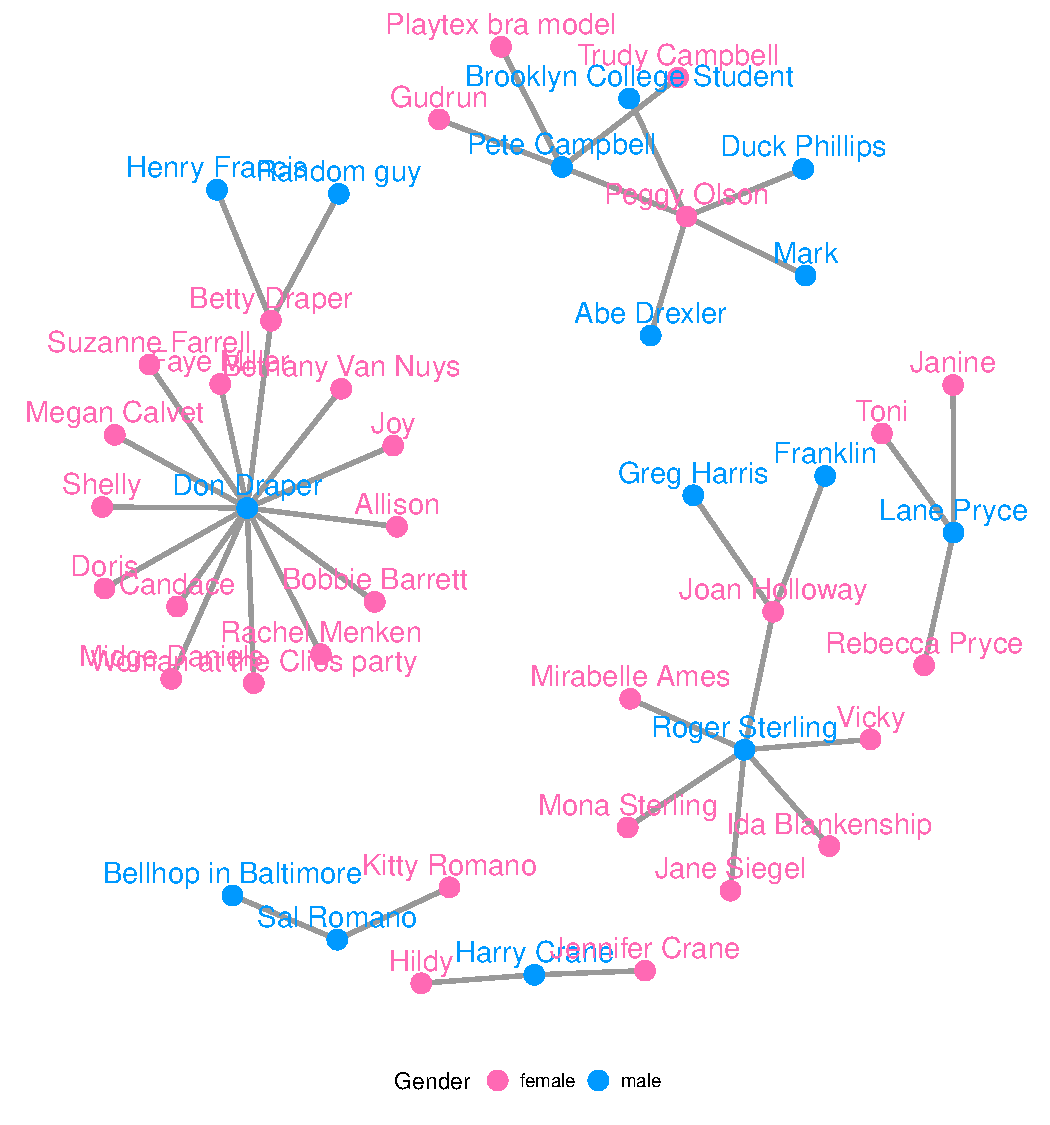
\includegraphics[width=0.6\textwidth]{figure/madmen_geom_net-1.pdf}
\caption{\label{fig.cap:madmen} Graph of the characters in the show Mad Men who are linked by a romantic relationship. }
\end{figure}

Figure~\ref{fig.cap:madmen} is a visualization of this network. In the plot, we can see one central character who has many more relationships than any other character. This vertex represents the main character of the show, Don Draper, who is quite the ``ladies' man." Networks like this one, no matter how simple or complex, are everywhere, and we hope to provide the curious reader with a straightforward way to visualize any network they choose.

Coloring the vertices or edges in a graph is a quick way to visualize grouping and helps with pattern or cluster detection. The vertices in a network and the edges between them compose the structure of a network, and being able to visually discover patterns among them is a key part of network analysis. Viewing multiple layouts of the same network can also help reveal patterns or clusters that would not be discovered when only viewing one layout or analyzing only its underlying adjacency matrix.

\section{Three implementations of network visualizations}%
\label{sec:implementations}

We present two basic approaches to using the \pkg{ggplot2} framework for network visualization. First, we implement network visualizations by providing a wrapper function, \code{ggnet2} for the user to visualize a network using \pkg{ggplot2} elements \citep{ggally}. Second, we implement network visualizations using layering in \pkg{ggplot2}.  For the second approach, we have two ways of creating a network visualization. The first, \pkg{geomnet}, wraps all network structures, including vertices, edges, and vertex labels into a single \code{geom}. The second, \pkg{ggnetwork}, implements each of these structural components in an independent \code{geom} and layers them to create the visualization \citep{ggnetwork}. In each package, our goal is to provide users with a way to map network properties to aesthetic properties of graphs that is familiar to them and straightforward to implement. Each package has a slightly different approach to accomplish this goal, and we will discuss all of these approaches in this section. For each implementation, we also provide the code necessary to create Figure~\ref{fig.cap:madmen}, and describe the arguments used. We conclude the section with a side-by-side comparison of the features available in all three implementations in Table~\ref{tab:comparison}.

\subsection{ggnet2} 

The \code{ggnet2} function is a part of the \pkg{GGally} package, a suite of functions developed to extend the plotting capabilities of \pkg{ggplot2} \citep{ggally}.  A detailed description of the \code{ggnet2} function is available from within the package as a vignette. Some example code to recreate Figure~\ref{fig.cap:madmen} using \code{ggnet2} is presented in Figure~\ref{fig.cap:madmenggnet2}. 

\begin{figure}[h]
\begin{knitrout}
\definecolor{shadecolor}{rgb}{1, 1, 1}\color{fgcolor}\begin{kframe}
\begin{verbatim}
library(GGally)
library(network)
# make the data available
data(madmen, package = 'geomnet')
# data step for both ggnet2 and ggnetwork
# create undirected network
mm.net <- network(madmen$edges[, 1:2], directed = FALSE)
mm.net # glance at network object
##  Network attributes:
##   vertices = 45 
##   directed = FALSE 
##   hyper = FALSE 
##   loops = FALSE 
##   multiple = FALSE 
##   bipartite = FALSE 
##   total edges= 39 
##     missing edges= 0 
##     non-missing edges= 39 
## 
##  Vertex attribute names: 
##     vertex.names 
## 
## No edge attributes
# create node attribute (gender)
rownames(madmen$vertices) <- madmen$vertices$label
mm.net %v% "gender" <- as.character(
  madmen$vertices[ network.vertex.names(mm.net), "Gender"]
)
# gender color palette
mm.col <- c("female" = "#ff69b4", "male" = "#0099ff")
# create plot for ggnet2
set.seed(10052016)
ggnet2(mm.net, color = mm.col[ mm.net %v% "gender" ],
       labelon = TRUE, label.color = mm.col[ mm.net %v% "gender" ],
       size = 2, vjust = -0.6, mode = "kamadakawai", label.size = 3)
\end{verbatim}
\end{kframe}
\end{knitrout}
\caption{\label{fig.cap:madmenggnet2} The code required to generate Figure~\ref{fig.cap:madmen} using the \code{ggnet2} function in the \pkg{GGally} package.}
\end{figure}

The \code{ggnet2} function offers a large range of network visualization functionality in a single function call. Although its result is a \pkg{ggplot2} object that can be further styled with \pkg{ggplot2} scales and themes, the syntax of the \code{ggnet2} function is designed to be easily understood by the users, who may not be familiar with \pkg{ggplot2} objects. The aesthetics relating to the nodes are controlled by arguments such as \code{node.alpha} or \code{node.color}, while those relating to the edges are controlled by arguments starting with \samp{edge}. Additionally, as seen in Figure~\ref{fig.cap:madmenggnet2}, the usual \pkg{ggplot2} arguments like \code{color} can be used without the prefix to map node attributes to aesthetic values. The arguments with the \code{node.} prefix are aliased versions for readability of the code. Thus, while \code{ggnet2} applies the grammar of graphics to network objects, the function itself still works very much like the plotting functions of the \pkg{igraph} and \pkg{network} packages: a long series of arguments is used to control every possible aspect of how the network should be visualized.

The \code{ggnet2} function takes a single network object as input. This initial object might be an object of class \code{"network"} from the \pkg{network} package (with the exception of hypergraphs or multiplex graphs), or any data structure that can be coerced to an object of that class via functions in the \pkg{network} package, such as an incidence matrix, an adjacency matrix, or an edge list. Additionally, if the \CRANpkg{intergraph} package \citep{intergraph} is installed, the function  also accepts a network object of class \code{"igraph"}. Internally, the function converts the network object to two data frames: one for edges and another one for nodes. It then passes them to \pkg{ggplot2}. Each of the two data frames contain the information required by \pkg{ggplot2} to plot segments and points respectively, such as a shape for the points (nodes) and a line type for the segments (edges). The final result returned to the user is a plot with a minimum of two layers, or more if there are edge and/or node labels.

The \code{mode} argument of \code{ggnet2} controls how the nodes of the network are to be positioned in the plot returned by the function. This argument can take any of the layout values supported by the \code{gplot.layout} function of the \pkg{sna} package, and defaults to \samp{fruchtermanreingold}, which places the nodes through the force-directed layout algorithm by \citet{fruchterman_reingold}. In the example presented in Figure~\ref{fig.cap:madmenggnet2}, the Kamada-Kawai layout is used by adding \samp{mode = "kamadakawai"} to the function call. Many other possible layouts and their parameters can also be passed to \code{ggnet2} through the \code{layout.par} argument. For a list of possible layouts and their arguments, see \code{?sna::gplot.layout}.

Other arguments passed to the \code{ggnet2} function offer extensive control over the aesthetics of the plot that it returns, including the addition of edge and/or node labels and their respective aesthetics. Arguments such as \code{node.shape} or \code{edge.lty}, which  control the shape of the nodes and the line type of the edges, respectively, can take a single global value, a vector of global values, or the name of an edge or vertex attribute to be used as an aesthetic mapping. This feature is used to change the size of the nodes and the node labels in Figure~\ref{fig.cap:madmenggnet2} by including \samp{size = 2} and \samp{label.size = 3} in the function call. 

This last functionality builds on one of the strengths of the \code{"network"} class, which can store information on network edges and nodes as attributes that are then accessible to the user through the \code{\%e\%} and \code{\%v\%} operators respectively.%
\footnote{See \citet[p.~22-24]{network}.
The equivalent operators in the \pkg{igraph} package are called \code{E} and \code{V}.} Usage examples of these operators can be seen in Figure~\ref{fig.cap:madmenggnet2}. The attribute of gender is assigned to nodes, which in turn is accessed to color the nodes and node labels by gender.  If the \code{ggnet2} function is given the \code{node.alpha = "importance"} argument, it will interpret it as an attempt to map the vertex attribute called \samp{importance} to the transparency level of the nodes. This works exactly like the command \code{net \%v\% "importance"}, which returns the vertex attribute \samp{importance} of the \code{"network"} object \code{net}. This functionality allows the \code{ggnet2} function to work in a similar fashion to \pkg{ggplot2} mappings of aesthetics within the \code{aes} operator.

The \code{ggnet2} function also provides a few network-specific options, such as sizing the nodes as a function of their unweighted degree, or using the primary and secondary modes of a bipartite network as an aesthetic mapping for the nodes. 

All in all, the \code{ggnet2} function combines two different kinds of processes: it translates a network object into a data frame suitable for plotting with \pkg{ggplot2}, and it applies network-related aesthetic operations to that data frame, such as coloring the edges in function of the color of the nodes that they connect. 

\subsection{geomnet} 

\begin{figure}[h]
\begin{knitrout}
\definecolor{shadecolor}{rgb}{1, 1, 1}\color{fgcolor}\begin{kframe}
\begin{verbatim}
# also loads ggplot2
library(geomnet)

# data step: join the edge and node data with a fortify call
MMnet <- fortify(as.edgedf(madmen$edges), madmen$vertices)
# create plot
set.seed(10052016)
ggplot(data = MMnet, aes(from_id = from_id, to_id = to_id)) +
  geom_net(aes(colour = Gender), layout.alg = "kamadakawai", 
           size = 2, labelon = TRUE, vjust = -0.6, ecolour = "grey60",
           directed =FALSE, fontsize = 3, ealpha = 0.5) +
  scale_colour_manual(values = c("#FF69B4", "#0099ff")) +
  xlim(c(-0.05, 1.05)) +
  theme_net() +
  theme(legend.position = "bottom")
\end{verbatim}
\end{kframe}
\end{knitrout}
\caption{\label{fig.cap:madmengeomnet} The code required to generate Figure~\ref{fig.cap:madmen} using the \code{geom\_net} function in the \pkg{geomnet} package.}
\end{figure}

\subsubsection{Data structure}

The package \pkg{geomnet} implements network visualization in a single \pkg{ggplot2} layer. A stable version is available on CRAN, with a development version available at \url{https://github.com/sctyner/geomnet}. The package has two main functions:  \code{stat\_net}, which performs all of the calculations, and \code{geom\_net}, which renders the plot. It also contains the secondary functions \code{geom\_circle} and \code{theme\_net}, which assist, respectively, in drawing self-referencing edges and removing axes and other background elements from the plots.
The approach in \pkg{geomnet} is similar to the implementation of other, native \pkg{ggplot2} geoms, such as \code{geom\_smooth}. When using \code{geom\_smooth}, the user does not need to know about any of the internals of the loess function, and similarly, when using \code{geomnet}, the user is not expected to know about the internals of the layout algorithm, just the name of the algorithm they'd like to use. On the other hand, if users are comfortable with network analysis, the entire body of layout methods provided by the \pkg{sna} package is available to them through the parameters \code{layout.alg} and \code{layout.par}.

In network analysis there are usually two sources of information: one data set consisting of a description of the nodes, represented as the vertices in the network and vertex attributes, and another data set detailing the relationship between these nodes, i.e.\ it consists of the edge list and any additional edge attributes. The minimum amount of information needed is a vector of all vertex labels and a two column data frame that encodes the edge list of the network. In order for this geometry to work, these two data sets need to be combined into a single data frame. For this, we implemented several new \code{fortify} methods for producing the correct data structure from different S3 objects that encode network information. Supported classes are \code{"network"} from the \pkg{sna} and \pkg{network} packages, \code{"igraph"} from the \pkg{igraph} package, \code{"adjmat"}, and \code{"edgedf"}. The last two are new classes introduced in \pkg{geomnet} that are identical to the \code{"matrix"} and \code{"data.frame"} classes, respectively. We created these new classes and the functions \code{as.adjmat()} and \code{as.edgedf()} so that network data in adjacency matrix and edgelist (data frame) formats can have their own fortify functions, separate from the very generic \code{"matrix"} and \code{"data.frame"} classes. These fortify functions combine the edge and the node information using a full join. A full join is used because generally, there will be some vertices that are sinks in the network because they only show up in the `to' column, and so we accommodate for these by adding artificial edges in the data set that have missing information for the `to' column. The user may also pass two data frames to the function, e.g.\ \samp{data = edge\_data} and \samp{vertices = vertex\_data}, but we recommend using the \code{fortify} methods whenever possible.

A usage example of the \code{fortify.edgedf} method is presented in Figure~\ref{fig.cap:madmengeomnet} with the creation of the \code{MMnet} data set. Two dataframes, \code{madmen\$edges} and \code{madmen\$vertices} are joined to create the required data. The first few rows of these data sets and their merged result are below. 

\begin{knitrout}
\definecolor{shadecolor}{rgb}{1, 1, 1}\color{fgcolor}\begin{kframe}
\begin{verbatim}
head(as.edgedf(madmen$edges), 3)
##        from_id         to_id
## 1 Betty Draper Henry Francis
## 2 Betty Draper    Random guy
## 3   Don Draper       Allison
head(madmen$vertices, 3)
##                     label Gender
## Betty Draper Betty Draper female
## Don Draper     Don Draper   male
## Harry Crane   Harry Crane   male
head(fortify(as.edgedf(madmen$edges), madmen$vertices), 3)
##        from_id         to_id Gender
## 1 Betty Draper Henry Francis female
## 2 Betty Draper    Random guy female
## 3   Don Draper       Allison   male
\end{verbatim}
\end{kframe}
\end{knitrout}

The formal requirements of \code{stat\_net} are two columns, called \code{from\_id} and \code{to\_id}. During this routine, columns \code{x, y} and \code{xend, yend} are calculated and used as a required input for \code{geom\_net}.

Other variables may also be included for each edge, such as the edge weight, in-degree, out-degree or grouping variable.

\subsubsection{Parameters and aesthetics}

Parameters that are currently implemented in \code{geom\_net} are:

\begin{itemize}
\item {\bf layout:}
the \code{layout.alg} parameter takes a character value corresponding to the possible network layouts in the \pkg{sna} package that are available within the \code{gplot.layout.*()} family of functions.  The default layout algorithm used is the Kamada-Kawai layout, a force-directed layout for undirected networks \citep{kamadakawai}.

In \pkg{sna}, for each layout there is a corresponding set of possible layout parameters, \code{layout.par}, which can be passed as a list to \code{geom\_net}. If the user wishes to create small multiples using \pkg{ggplot2} \code{facets}, they can use \code{fiteach}, a logical value specifying whether the same layout should be used for all panels (default) or each panel's data should be fit separately. Finally, the \code{singletons} parameter is a logical value that dictates whether or not to include nodes with zero indegree and zero outdegree in the visualization. The default is set to \code{TRUE}, and if set to \code{FALSE} nodes will only appear in panels where they have indegree or outdegree of at least one. 
\item {\bf vertices:} any of \pkg{ggplot2}'s aesthetics relating to points: \code{colour}, \code{size}, \code{shape}, \code{alpha}, \code{x}, and \code{y} are available and used for specifying the appearance of nodes in the network. For example \samp{aes(colour = Gender)} is used in Figure~\ref{fig.cap:madmengeomnet} to color the nodes and node labels according to the gender of each character. 

\item {\bf edges:} for edges we distinguish between two different sets of aesthetics: aesthetics that only relate to line attributes, such as  \code{linewidth} and \code{linetype}, and aesthetics that are also used by the point \code{geom}.  The former can be used in the same way as they are used in \code{geom\_segment}, while the latter, like \code{alpha} or \code{colour}, for instance, are used for vertices unless separately specified. Instead, use the parameters \code{ecolour} or \code{ealpha}, which are only applied to the edges. If the \code{group} variable is specified, a new variable, called \code{samegroup} is added during the layout process. This variable is \code{TRUE}, if an edge is between two vertices of the same group, and \code{FALSE} otherwise. If \code{samegroup} is \code{TRUE}, the corresponding edge will be colored using the same color as the vertices it connects. If the edge is between vertices of a different group, the default grey shade is used for the edge.

The parameter \code{curvature} is set to zero by default, but if specified, leads to curved edges using the newly implemented \pkg{ggplot2} geom \code{geom\_curve} instead of the regular \code{geom\_segment}.
Note that the edge specific aesthetics that overwrite node aesthetics are currently considered as `as.is' values: they do not get a legend and are not scaled within the ggplot2 framework. This is done to avoid any clashes between node and edge scales.

{\bf self-referencing vertices:} some networks contain self references, i.e.\  an edge has the same vertex id in its from and to columns. If the parameter \code{selfloops} is set to \code{TRUE}, a circle is drawn using the new \code{geom\_circle} next to the vertex to represent this self reference.

\item {\bf arrow:} whenever the parameter \code{directed} is set from its default state to \code{TRUE}, arrows are drawn from the `from' to the `to' node, with tips pointing towards the `to' node.  By default, arrows have an absolute size of 10 points. The entire structure of the arrow can be changed by passing an \code{arrow} object from the \CRANpkg{grid} package to the \code{arrow} argument. If the user doesn't wish to change the whole arrow object, the parameters \code{arrowsize} and \code{arrowgap} are also available. The \code{arrowsize} argument is of a positive numeric value that is used as a multiple of the original arrow size, i.e.\ \code{arrowsize = 2} shows arrow tips at twice their original size.  The parameter \code{arrowgap} can be used to avoid overplotting of the arrow tips by the nodes, \code{arrowgap} specifies a proportion by which the edge should be shrunk with default of 0.05. A value of 0.5 will result in edges drawn only half way from the `from' node to the `to' node.
\item {\bf labels:}  the \code{labelon} argument is a logical parameter, which when set to \code{TRUE} will label the nodes with their IDs, as is in Figure~\ref{fig.cap:madmen}. The \code{aes} option \code{label} can also be used to label nodes, in which case the nodes are labeled with the value corresponding to their respective values of the provided variable. If \code{colour} is specified for the nodes, the same values are used for the labels, unless \code{labelcolour} is specified. If \code{fontsize} is specified, it changes the label size to that value in points. Other parameter values, such as \code{vjust} and \code{hjust} help in adjusting labels relative to the nodes. The parameters work in the same fashion as in native \pkg{ggplot2} \code{geom}s. Additionally, the label can be drawn by using \code{geom\_text} (the default) or using the new \code{geom\_label} in \pkg{ggplot2} by adding \samp{labelgeom = "label"} to the arguments in \code{geom\_net}. Finally, with the help of the package \CRANpkg{ggrepel} by \citet{ggrepel} we have implemented the logical \code{repel} argument, which when true, uses \code{geom\_text\_repel} or \code{geom\_label\_repel} to plot the labels instead of \code{geom\_text} or \code{geom\_label}, respectively. Using \code{repel} can be extremely useful when the networks are dense or the labels are long, as in Figure~\ref{fig.cap:madmen}, helping to solve a common problem with many network visualizations. 

\end{itemize}

\subsection{ggnetwork} 

\pkg{ggnetwork} is a small R package that mimics the behavior of \code{geomnet} by defining several geoms to achieve similar results. 

\begin{figure}[h]
\begin{knitrout}
\definecolor{shadecolor}{rgb}{1, 1, 1}\color{fgcolor}\begin{kframe}
\begin{verbatim}
# create plot for ggnetwork. uses same data created for ggnet2 function
library(ggnetwork)
set.seed(10052016)
ggplot(data = ggnetwork(mm.net, layout = "kamadakawai"), 
       aes(x, y, xend = xend, yend = yend)) +
  geom_edges(color = "grey50") + # draw edge layer
  geom_nodes(aes(colour = gender), size = 2) + # draw node layer
  geom_nodetext(aes(colour = gender, label = vertex.names),
                size = 3, vjust = -0.6) + # draw node label layer
  scale_colour_manual(values = mm.col) +
  xlim(c(-0.05, 1.05)) +
  theme_blank() +
  theme(legend.position = "bottom")
\end{verbatim}
\end{kframe}
\end{knitrout}
\caption{\label{fig.cap:madmenggnetwork} The code required to generate Figure~\ref{fig.cap:madmen} using the \pkg{ggnetwork} package.}
\end{figure}

The approach taken by the \pkg{ggnetwork} package is to alias some of the native geoms of the \pkg{ggplot2} package. An aliased geom is simply a variant of an already existing one. The \pkg{ggplot2} package contains several examples of aliased geoms, such as \code{geom\_histogram}, which is a variant of \code{geom\_bar} see \citep[see][p.~67, Table~4.6]{ggplot2}.

Following that logic, the \pkg{ggnetwork} package adds four aliased geometries to \pkg{ggplot2}:

\begin{itemize}
  \item \code{geom\_nodes}, an alias to \code{geom\_point};
  \item \code{geom\_edges}, an alias to either \code{geom\_segment} or \code{geom\_curve};
  \item \code{geom\_nodetext}, an alias to \code{geom\_text}; and
  \item \code{geom\_edgetext}, an alias to \code{geom\_label}.
\end{itemize}

The four geoms are used to plot nodes, edges, node labels and edge labels, respectively. Two of the geoms that they alias, \code{geom\_curve} and \code{geom\_label}, are part of the new geometries introduced in \pkg{ggplot2} version 2.1.0. All four geoms behave exactly like those that they alias, and take exactly the same arguments. The only exception to that rule is the special case of \code{geom\_edges}, which accepts both the arguments of \code{geom\_segment} and those of \code{geom\_curve}; if its \code{curvature} argument is set to anything but \code{0} (the default), then \code{geom\_edges} behaves exactly like \code{geom\_curve}; otherwise, it behaves exactly like \code{geom\_segment}. Three of the four availble aliased \code{geom}s are used in Figure~\ref{fig.cap:madmenggnetwork} to create the visualization of the Mad Men relationship network. 

Just like the \code{ggnet2} function, the \pkg{ggnetwork} package takes a single network object as input. This can be an object of class \code{"network"}, some data structure coercible to that class, or an object of class \code{"igraph"} when the \pkg{intergraph} package is installed. This object is passed to the `workhorse' function of the package, which is also called \code{ggnetwork} to create a data frame, and then to the \code{data} argument of \code{ggplot()}.

Internally, the \code{ggnetwork} function starts by computing the \code{x} and \code{y} coordinates of all nodes in the network with respect to its \code{layout} argument, which defaults to the Fruchterman-Reingold layout algorithm \citep{fruchterman_reingold}. It then extracts the edge list of the network, to which it adds the coordinates of the sender and receiver nodes as well as all edge-level attributes. The result is a data frame with as many rows as there are edges in the network, and where the \code{x}, \code{y}, \code{xend} and \code{yend} hold the coordinates of the network edges.

At that stage, the \code{ggnetwork} function, like the \pkg{geomnet} package, performs a left-join of that augmented edge list with the vertex-level attributes of the %sender
`from' nodes. It also adds one self-loop per node, in order to ensure that every node is plotted even when their degree is zero---that is, even if the node is not connected to any other node of the network, and is therefore absent from the edge list. The data frame created by this process contains one row per edge as well as one additional row per node, and features all edge-level and vertex-level attributes initially present in the network.%
\footnote{One limitation of this process is that it requires some reserved variable names (\code{x}, \code{y}, \code{xend} and \code{yend}), which should not also be present as edge-level or vertex-level attributes (otherwise the function will simply break). Similarly, if an edge attribute and a vertex attribute have the same name, like  \samp{na}, which the \pkg{network} package defines as an attribute for both edges and vertices in order to flag missing data, \code{ggnetwork} will rename them to \samp{na.x} (for the edge-level attribute) and \samp{na.y} (for the vertex-level attribute).} 

The \code{ggnetwork} function also accepts the arguments \code{arrow.gap} and \code{by}. Like in \pkg{geomnet}, \code{arrow.gap} slightly shortens the edges of directed networks in order to avoid overplotting edge arrows and nodes. The argument \code{by} is intended for use with plot facets. Passing an edge attribute as a grouping variable to the \code{by} argument will cause \code{ggnetwork} to return a data frame in which each node appears as many times as there are unique values of that edge attribute, using the same coordinates for all occurrences. When that same edge attribute is also passed to either \code{facet\_wrap} or \code{facet\_grid}, each edge of the network will show in only one panel of the plot, and all nodes will appear in each of the panels at the same position. This makes the panels of the plot comparable to each other, and allows the user to visualize the network structure as a function of a specific edge attribute, like a temporal attribute.

\begin{table}
\begin{tabu} to \linewidth { X[l]| X[c] | X[c] | X[c] }
\toprule
& \code{ggnet2} & \code{geom\_net} & \code{geom\_nodes}, \code{geom\_edges}, etc\\
Functionality & (\pkg{GGally}) & (\pkg{geomnet}) &  (\pkg{ggnetwork}) \\
\midrule
Data &  object of class \code{"network"} or object easily converted to that class (i.e.\ incidence or adjacency matrices, edge list) or object of class \code{"igraph"} & a fortified \code{"network"}, \code{"igraph"}, \code{"edgedf"}, or \code{"adjmat"} object OR one edge data frame and one node data frame to be merged internally & same as \code{ggnet2}\\
\midrule
Naming conventions & \code{node.\_},  \code{edge.\_}, \code{label.\_}, \code{edge.label.\_} for \code{alpha}, \code{color}, etc.\ & arguments identical to \pkg{ggplot2} with exception of \code{ecolor}, \code{ealpha} & same as \pkg{ggplot2}\\
\midrule
Layout package \& default & \pkg{sna}, Fruchterman-Reingold & \pkg{sna}, Kamada-Kawai & \pkg{sna}, Fruchterman-Reingold\\
\midrule
Aesthetic mappings to variables & all \code{alpha}, \code{color}, \code{shape}, \code{size} for nodes, edges, labels & \code{colour}, \code{size}, \code{shape}, \code{x}, \code{y}, \code{linetype}, \code{linewidth}, \code{label}, \code{group}, \code{fontsize} & same as \pkg{ggplot2} \\
\midrule
Arrows & \code{directed = TRUE}, \code{arrow.size}, \code{gap} & \code{arrowsize}, \code{gap}, \code{arrow = arrow()} like \pkg{ggplot2} & specify arrows in \code{geom\_edge} like in code{geom\_segment}, \code{arrow.gap} \\
\midrule
Theme or palette changes & done in the function with arguments like \code{\_.legend}, \code{\_.palette}, etc.\ and adding \pkg{ggplot2} elements  & adding \pkg{ggplot2} elements & adding \pkg{ggplot2} elements \\
\midrule
Creating small multiples  & created separately, use \code{grid.arrange} from \pkg{gridExtra} & add \code{group} argument to \code{fortify()} and use \code{facet\_*()} from \pkg{ggplot2} & use \code{by} argument in \code{ggnetwork()} and \code{facet\_*()} from \pkg{ggplot2}\\
\midrule
Edge labelling? & Yes  & No & Yes\\
\midrule
Draw self-loops? &  No & Yes & No \\
\bottomrule
\end{tabu}
\caption{\label{tab:comparison} Comparing the three different package side-by-side. }
\end{table}

\section{Examples}
\label{sec:examples}

In this section, we demonstrate some of the current capabilities of \code{ggnet2}, \pkg{geomnet}, and \pkg{ggnetwork} in a series of side by side examples. While the output is nearly identical for each method of network visualization, the code and implementations differ across the three methods. For each of these examples, we present the code necessary to produce the network visualization in each of the three packages, and discuss each application in detail.

For the following examples we will be loading all three packages under comparison. In practice, only one of these packages would be needed to visualize a network in the \pkg{ggplot2} framework:
\begin{knitrout}
\definecolor{shadecolor}{rgb}{1, 1, 1}\color{fgcolor}\begin{kframe}
\begin{verbatim}
library(ggplot2)
library(GGally)
library(geomnet)
library(ggnetwork)
\end{verbatim}
\end{kframe}
\end{knitrout}

\subsection{Blood donation} 

We begin with a very simple example that most should be familiar with: blood donation. In this directed network, there are eight vertices and 27 edges.  The vertices represent the eight different blood types in humans that are most important for donation: the ABO blood types A, B, AB, and O, combined with the RhD positive (+) and negative (-) types. The edges are directed: a person whose blood type is that of a \emph{from} vertex can to donate blood to a person whose blood type is that of a corresponding \emph{to} vertex.  This network is shown in Figure~\ref{fig.cap:blood}. The code to produce each one of the networks is shown above Figure~\ref{fig.cap:blood}. We take advantage of each approach's ability to assign identity values to the aesthetic values. The color is changed to a dark red, the size of the nodes is changed to be large enough to accomodate the blood type label, which we also change the color of, and we use the directed and arrow arguments of each implementation to show the precise blood donation relationships. Additionally, we change the node layout to circle, and the placement of the labels with the \code{hjust} and \code{vjust} options. 

\begin{knitrout}
\definecolor{shadecolor}{rgb}{1, 1, 1}\color{fgcolor}\begin{kframe}
\begin{verbatim}
# make data accessible
data(blood, package = "geomnet")

# plot with ggnet2 (Figure 5a)
set.seed(12252016)
ggnet2(network(blood$edges[, 1:2], directed=TRUE), 
       mode = "circle", size = 15, label = TRUE, 
       arrow.size = 10, arrow.gap = 0.05, vjust = 0.5,
       node.color = "darkred", label.color = "grey80")
\end{verbatim}
\end{kframe}
\end{knitrout}

\begin{knitrout}
\definecolor{shadecolor}{rgb}{1, 1, 1}\color{fgcolor}\begin{kframe}
\begin{verbatim}
head(blood$edges,3) # glance at the data
##   from  to group_to
## 1  AB- AB+     same
## 2  AB- AB-     same
## 3  AB+ AB+     same
# plot with geomnet (Figure 5b)
set.seed(12252016)
ggplot(data = blood$edges, aes(from_id = from, to_id = to)) +
  geom_net(colour = "darkred", layout.alg = "circle", labelon = TRUE, size = 15,
           directed = TRUE, vjust = 0.5, labelcolour = "grey80",
           arrowsize = 1.5, linewidth = 0.5, arrowgap = 0.05,
           selfloops = TRUE, ecolour = "grey40") + 
  theme_net() 
\end{verbatim}
\end{kframe}
\end{knitrout}

\begin{knitrout}
\definecolor{shadecolor}{rgb}{1, 1, 1}\color{fgcolor}\begin{kframe}
\begin{verbatim}
# plot with ggnetwork (Figure 5c)
set.seed(12252016)
ggplot(ggnetwork(network(blood$edges[, 1:2]),
                 layout = "circle", arrow.gap = 0.05),
       aes(x, y, xend = xend, yend = yend)) +
  geom_edges(color = "grey50",
             arrow = arrow(length = unit(10, "pt"), type = "closed")) +
  geom_nodes(size = 15, color = "darkred") +
  geom_nodetext(aes(label = vertex.names), color = "grey80") +
  theme_blank()
\end{verbatim}
\end{kframe}
\end{knitrout}
\noindent
In this example every vertex has a self-reference, as blood between two people of matching ABO and RhD type can always be exchanged.  The \pkg{geomnet} approach shows these self-references as circles looping back to the vertex, which is controlled by using the parameter setting \code{selfloops = TRUE}.

\begin{figure}[hbt]
\begin{subfigure}[t]{.32\textwidth}
\caption{ggnet2}
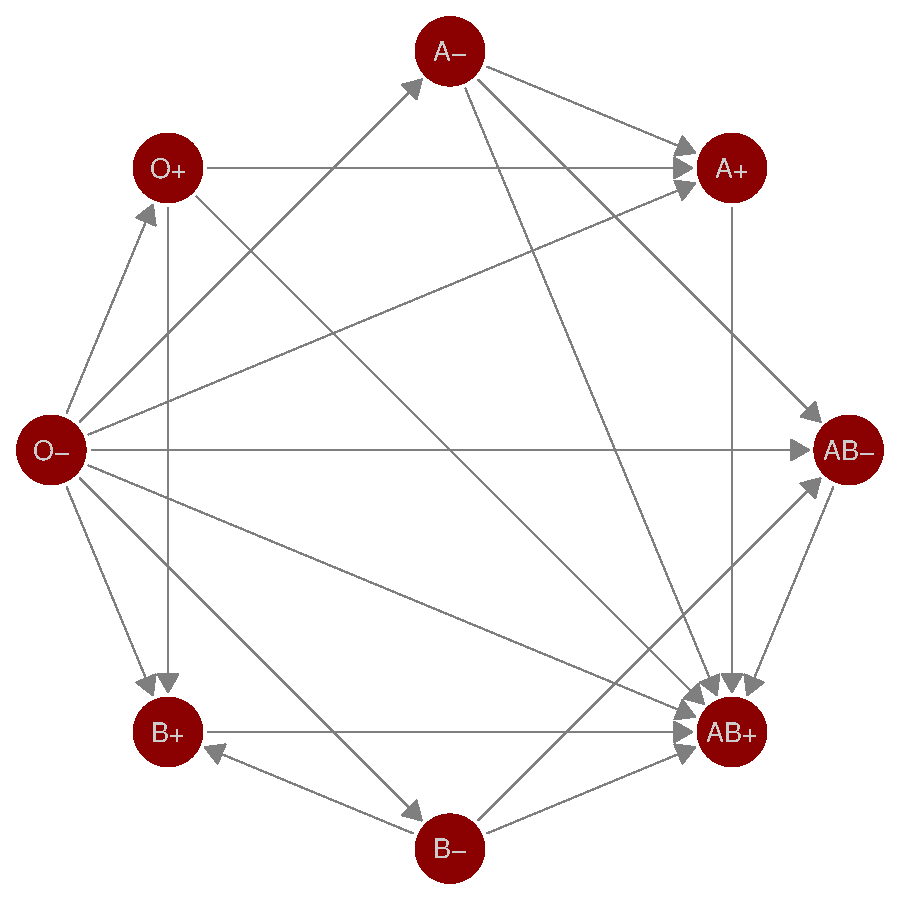
\includegraphics[width=\textwidth]{figure/blood_ggnet2-1.pdf}
\end{subfigure}
\begin{subfigure}[t]{.32\textwidth}
\caption{geomnet}
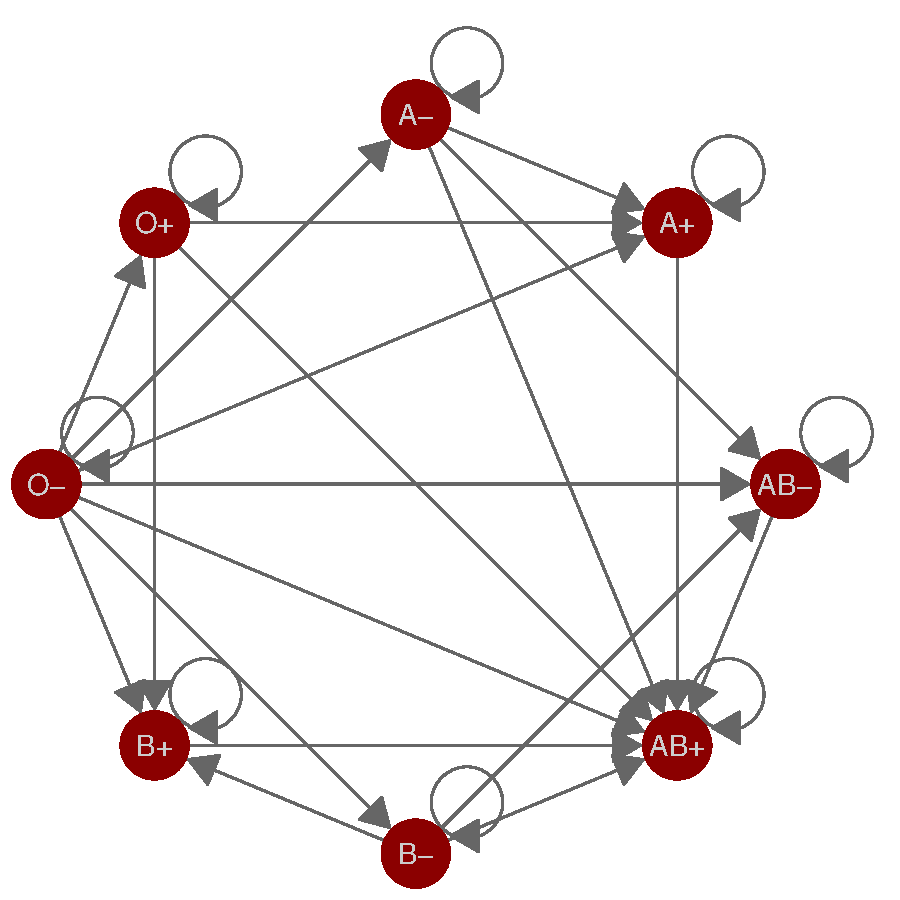
\includegraphics[width=\textwidth]{figure/blood_geom_net-1.pdf}
\end{subfigure}
\begin{subfigure}[t]{.32\textwidth}
\caption{ggnetwork}
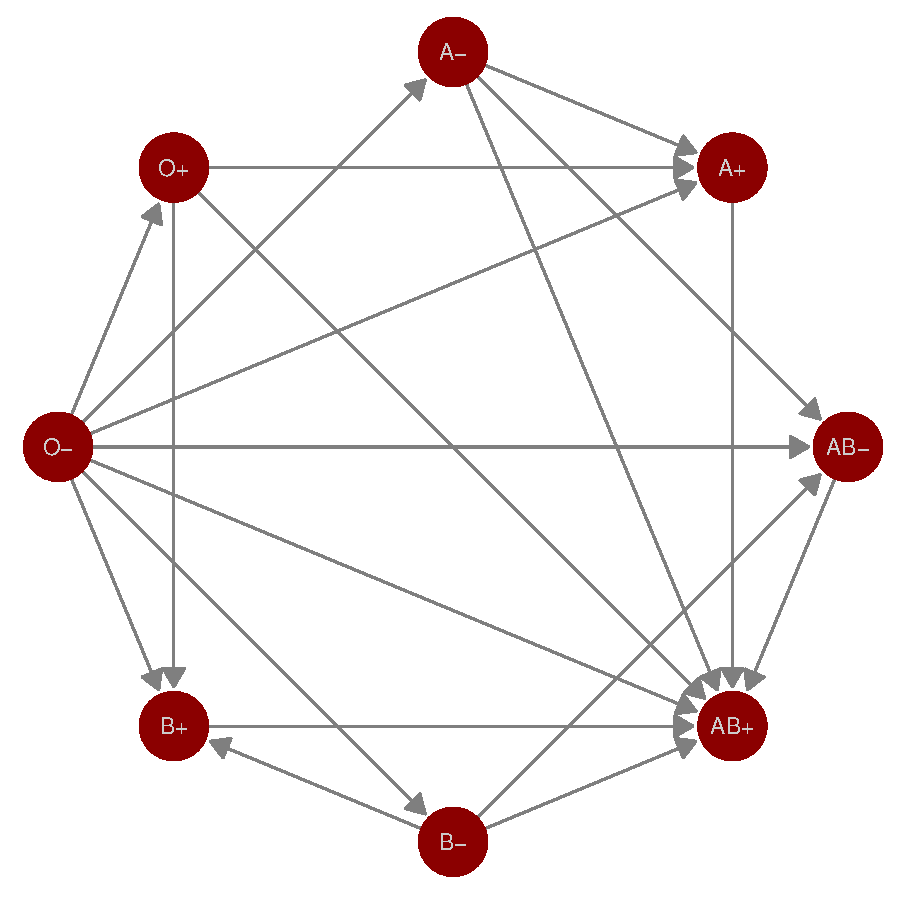
\includegraphics[width=\textwidth]{figure/blood_ggnetwork-1.pdf}
\end{subfigure}
\caption{\label{fig.cap:blood} Network of blood donation possibilities in humans by ABO and RhD blood types.}
\end{figure}

\code{colour} and \code{size} aesthetics in Figure~\ref{fig.cap:blood} are set to identity values to change the size and color of all vertices. We have also used the \code{layout} and \code{label} arguments to change the default Kamada-Kawai layout to a circle layout and to print labels for each of the blood types. The circle layout places blood types of the same ABO type next to each other and spreads the vertices out far enough to distinguish between the various ``in" and ``out" types.  We can tell clearly from this plot that the O-type is the universal donor: it has an out-degree of seven and an in-degree of zero. Additionally, we can see that the AB+ type is the universal recipient, with an in-degree of seven and an out-degree of zero. Anyone looking at this plot can quickly determine which type(s) of blood they can receive and which type(s) can receive their blood.

\subsection{Email network} 

\begin{figure}[hbt]
\begin{subfigure}[t]{\textwidth}
\caption{ggnet2}
\vspace{1em}

             \begin{adjustbox}{valign=t}

             \begin{minipage}{.49\textwidth}
 \begin{knitrout}\footnotesize
\definecolor{shadecolor}{rgb}{1, 1, 1}\color{fgcolor}\begin{kframe}
\begin{verbatim}
# make data accessible
data(email, package = 'geomnet')

# create node attribute data
em.cet <- as.character(
  email$nodes$CurrentEmploymentType)
names(em.cet) = email$nodes$label

# remove the emails sent to all employees
edges <- subset(email$edges, nrecipients < 54)
# create network
em.net <- edges[, c("From", "to") ]
em.net <- network(em.net, directed = TRUE)
# create employee type node attribute
em.net %v% "curr_empl_type" <-
  em.cet[ network.vertex.names(em.net) ]
set.seed(10312016)
ggnet2(em.net, color = "curr_empl_type",
       size = 4, palette = "Set1", arrow.gap = 0.02,
       arrow.size = 5, edge.alpha = 0.25, 
       mode = "fruchtermanreingold",
       edge.color = c("color", "grey50"),
       color.legend = "Employment Type") +
  theme(legend.position = "bottom")
\end{verbatim}
\end{kframe}
\end{knitrout} \vspace{1em}

                   \end{minipage}

                  \begin{minipage}{.49\textwidth}

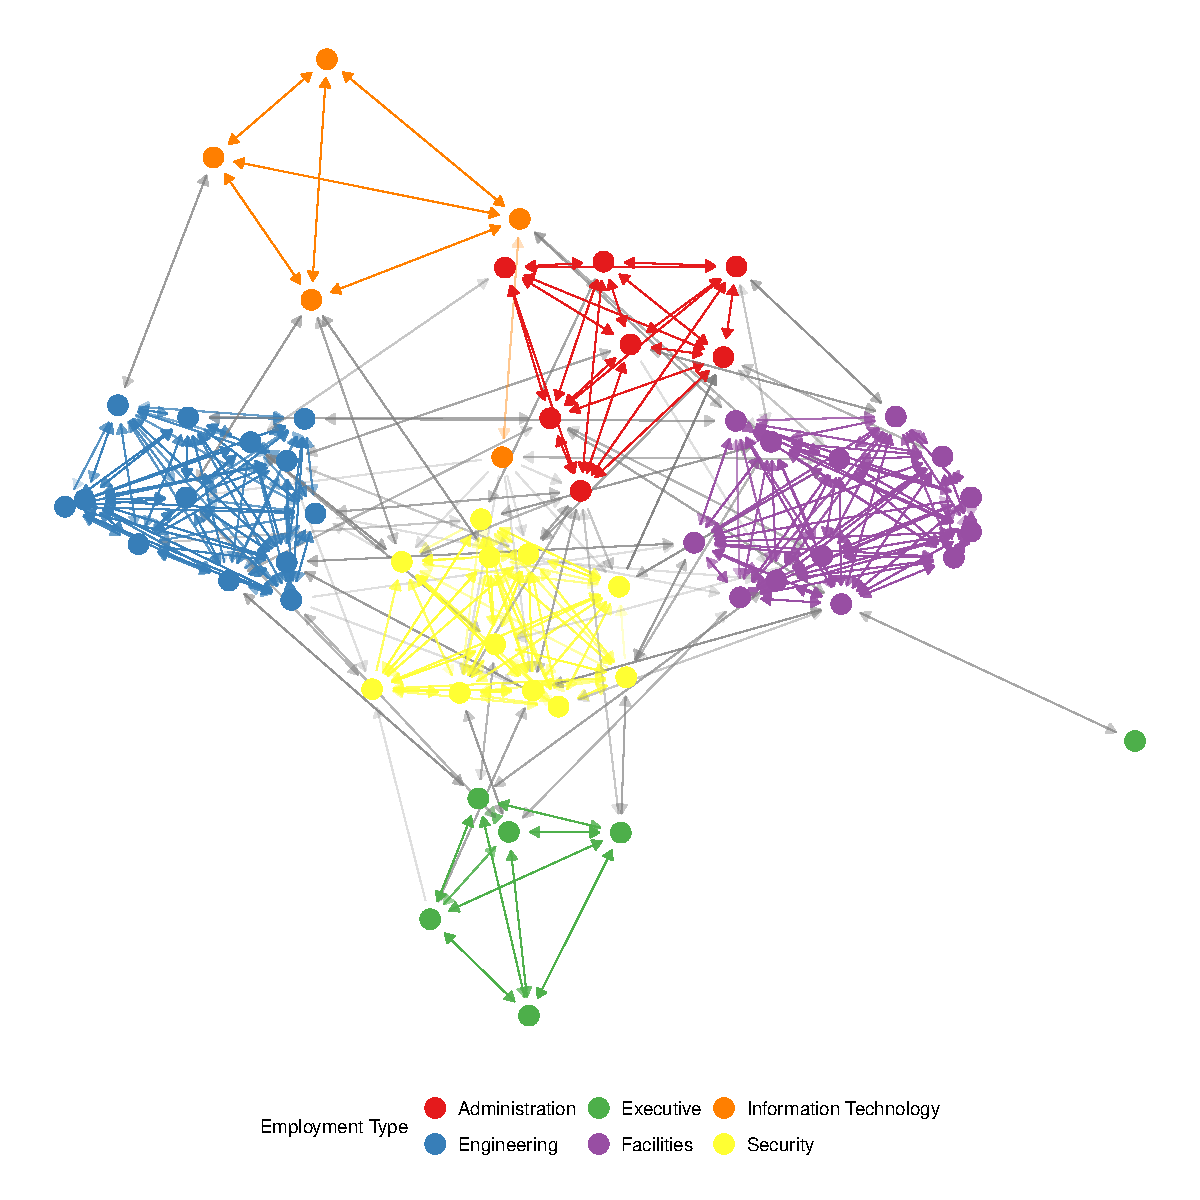
\includegraphics[width=\textwidth]{figure/email_ggnet2-1.pdf}

                          \end{minipage}

                          \end{adjustbox}

\end{subfigure}

\begin{subfigure}[t]{\textwidth}
\caption{geomnet}
\vspace{1em}

             \begin{adjustbox}{valign=t}

             \begin{minipage}{.49\textwidth}
 \begin{knitrout}\footnotesize
\definecolor{shadecolor}{rgb}{1, 1, 1}\color{fgcolor}\begin{kframe}
\begin{verbatim}
# data step for the geomnet plot
email$edges <- email$edges[, c(1,5,2:4,6:9)]
emailnet <- fortify(
  as.edgedf(subset(email$edges, nrecipients < 54)),
  email$nodes)
set.seed(10312016)
ggplot(data = emailnet,
       aes(from_id = from_id, to_id = to_id)) +
  geom_net(layout.alg = "fruchtermanreingold",
    aes(colour = CurrentEmploymentType,
        group = CurrentEmploymentType,
        linewidth = 3 * (...samegroup.. / 8 + .125)),
    ealpha = 0.25, size = 4, curvature = 0.05,
    directed = TRUE, arrowsize = 0.5) +
  scale_colour_brewer("Employment Type", palette = "Set1") +
  theme_net() +
  theme(legend.position = "bottom")
\end{verbatim}
\end{kframe}
\end{knitrout} \vspace{1em}

                   \end{minipage}

                  \begin{minipage}{.49\textwidth}

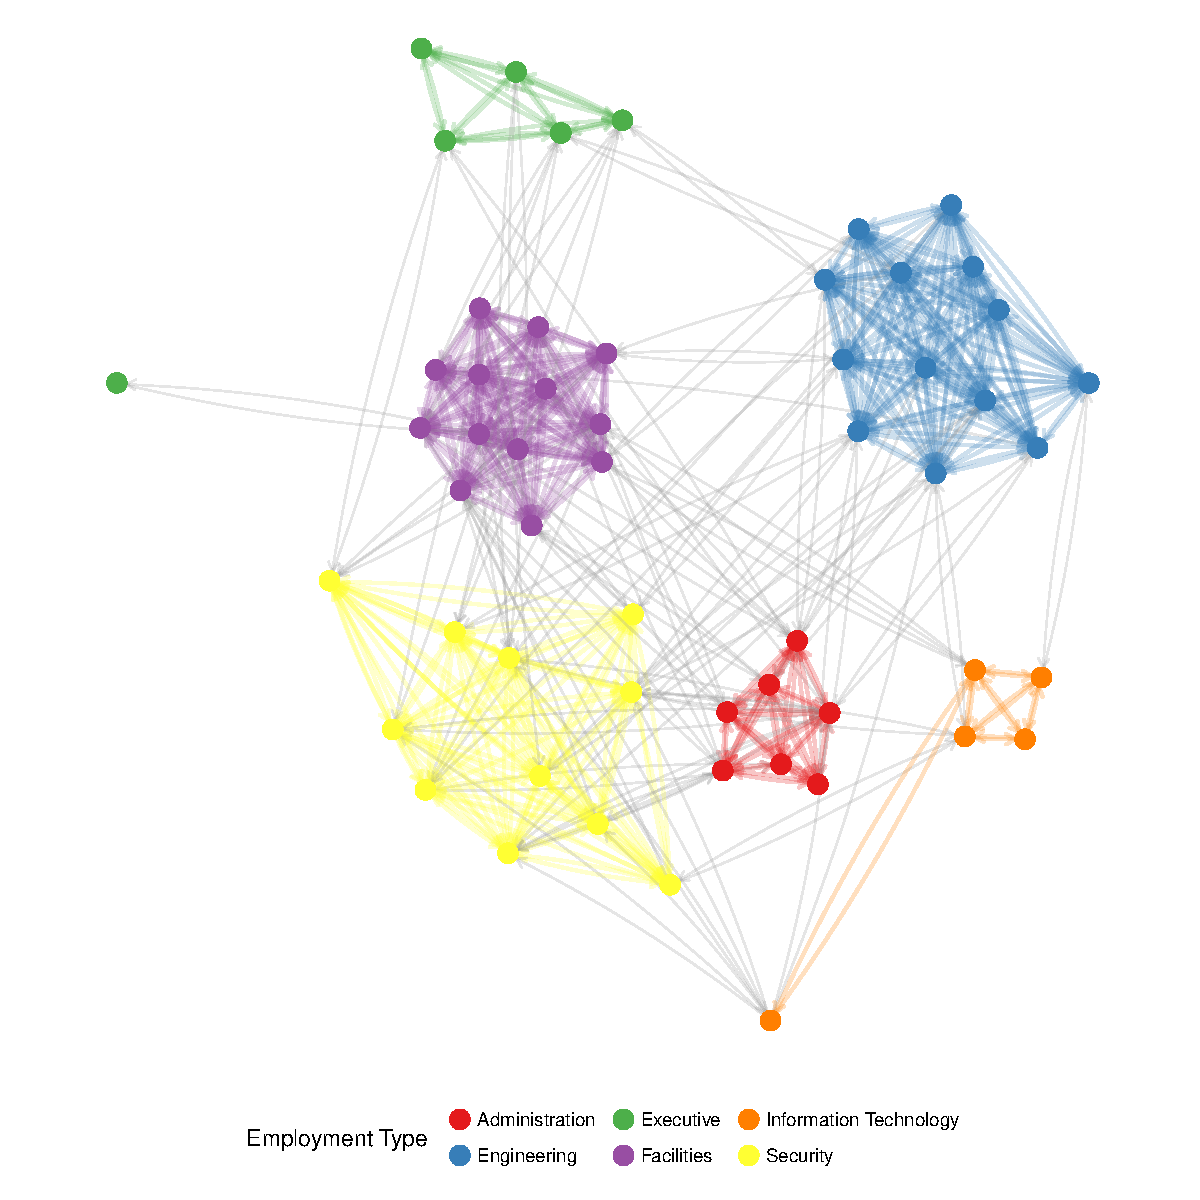
\includegraphics[width=\textwidth]{figure/email_geom_net-1.pdf}

                          \end{minipage}

                          \end{adjustbox}
\end{subfigure}

\begin{subfigure}[t]{\textwidth}
\caption{ggnetwork}
\vspace{1em}

             \begin{adjustbox}{valign=t}

             \begin{minipage}{.49\textwidth}
 \begin{knitrout}\footnotesize
\definecolor{shadecolor}{rgb}{1, 1, 1}\color{fgcolor}\begin{kframe}
\begin{verbatim}
# use em.net created in ggnet2step
set.seed(10312016)
ggplot(ggnetwork(em.net, arrow.gap = 0.02,
              layout = "fruchtermanreingold"),
       aes(x, y, xend = xend, yend = yend)) +
  geom_edges(
    aes(color = curr_empl_type),
    alpha = 0.25,
    arrow = arrow(length = unit(5, "pt"),
                  type = "closed"),
    curvature = 0.05) +
  geom_nodes(aes(color = curr_empl_type),
             size = 4) +
  scale_color_brewer("Employment Type",
                     palette = "Set1") +
  theme_blank() +
  theme(legend.position = "bottom")
\end{verbatim}
\end{kframe}
\end{knitrout} \vspace{1em}

                   \end{minipage}

                  \begin{minipage}{.49\textwidth}

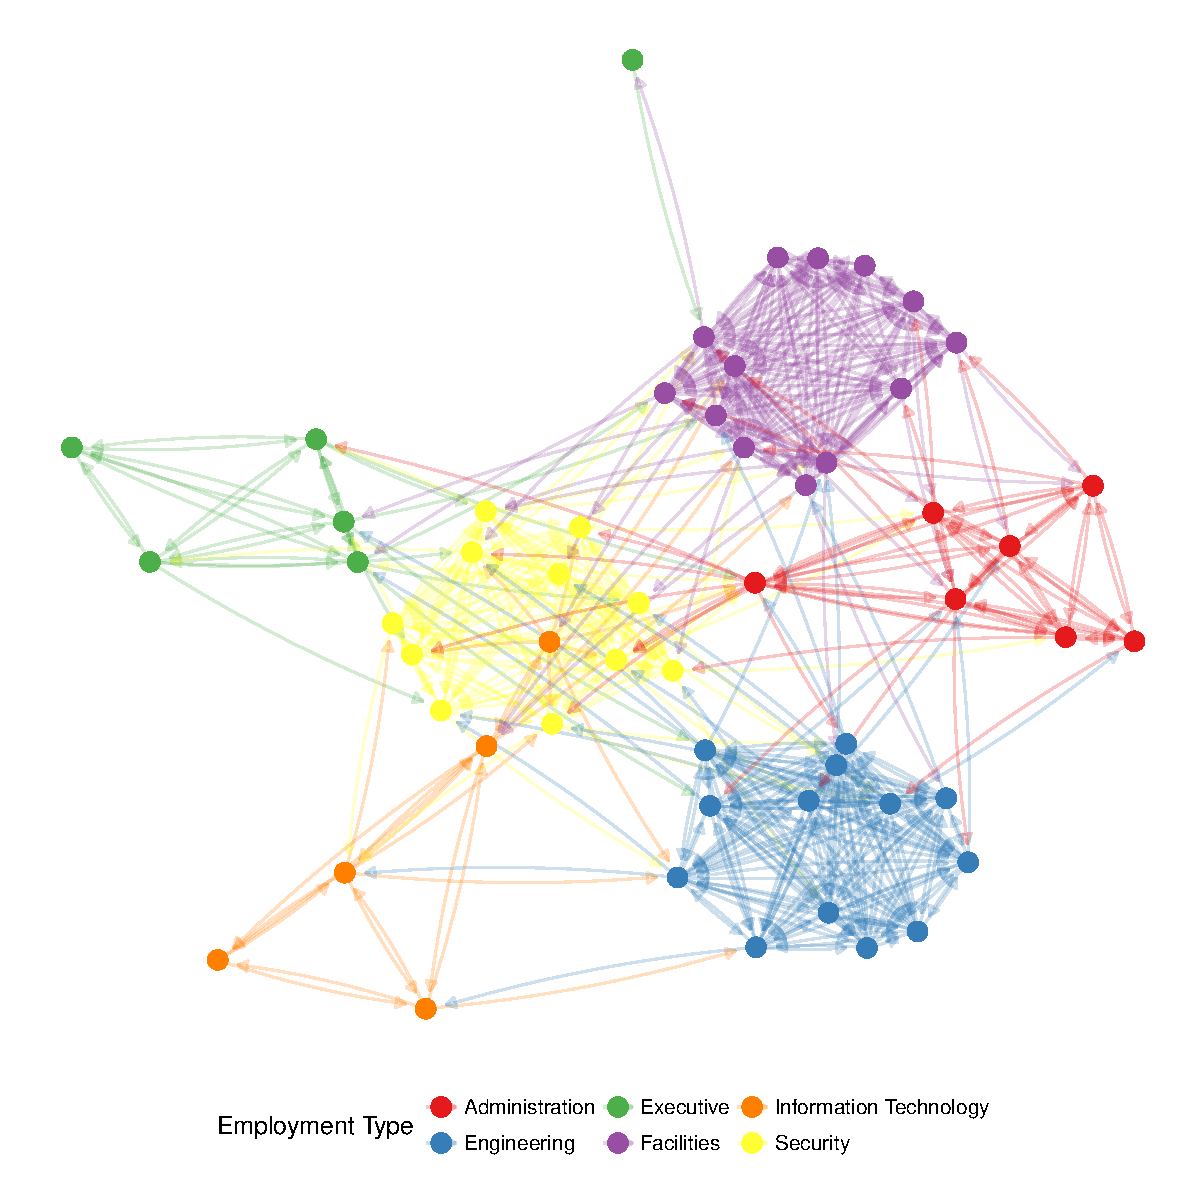
\includegraphics[width=\textwidth]{figure/email_ggnetwork-1.pdf}

                          \end{minipage}

                          \end{adjustbox}
\end{subfigure}

\caption{\label{fig.cap:email} Email network within a company over a two week period.}
\end{figure}
\afterpage{\clearpage}

The email network comes from the 2014 VAST Challenge \citep{emailnet}. It is a directed network of emails between company employees with 55 vertices and 9,063 edges. Each vertex represents an employee of the company, and each edge represents an email sent from one employee to another. The arrow of the directed edge points to the recipient of the email. If an email has multiple recipients, multiple edges, one for each recipient, are included in the network. The network contains two business weeks of emails across the entire company. In order to better visualize the structure of the communication network between employees, emails that were sent out to all employees are removed. A glimpse of the data objects used is below. 

\begin{knitrout}
\definecolor{shadecolor}{rgb}{1, 1, 1}\color{fgcolor}\begin{kframe}
\begin{verbatim}
em.net # ggnet2 and ggnetwork
##  Network attributes:
##   vertices = 55 
##   directed = TRUE 
##   hyper = FALSE 
##   loops = FALSE 
##   multiple = FALSE 
##   bipartite = FALSE 
##   total edges= 4743 
##     missing edges= 0 
##     non-missing edges= 4743 
## 
##  Vertex attribute names: 
##     curr_empl_type vertex.names 
## 
##  Edge attribute names not shown
emailnet[1,c(1:2,7,21)] # geomnet
##                                 from_id
## 1 Ada.Campo-Corrente@gastech.com.kronos
##                                to_id day
## 1 Ingrid.Barranco@gastech.com.kronos  10
##   CurrentEmploymentType
## 1             Executive
\end{verbatim}
\end{kframe}
\end{knitrout}

Emails taken by themselves form an event network, i.e.\ edges do not have any temporal duration. Here, however, we can think of emails as observable expressions of the underlying, unobservable, relationship between employees. We can think of this network as a dynamic temporal network, i.e.\ this network has the potential to change over time. The \CRANpkg{ndtv} package by \cite{ndtv} allows the analysis of such networks and provides impressive animations of the underlying dynamics. 
Here, we are using two static approaches to visualize the network: first, we aggregate emails across the whole time frame (shown in Figure~\ref{fig.cap:email}), then we  
aggregate emails by day and use small multiples to allow a comparison of day-to-day behavior (shown in Figure~\ref{fig:email_facet}).

For all of the email examples, we have colored the vertices by the variable \code{CurrentEmploymentType}, which contains the department in the company of which each employee is a part of. There are six distinct clusters in this network which almost perfectly correspond to the six different types of employees in this company: administration, engineering, executive, facilities, information technology, and security. Other features in the code include using \code{alpha} arguments to change the transparency of the edges, \code{curvature} argumnets to show mutual communication as two edges instead of one edge with two arrowheads, and the addition of \pkg{ggplot2} functions like \code{scale\_colour\_brewer} and \code{theme} to customize the colors of the nodes and their corresponding legend. 

In Figure~\ref{fig.cap:email} 
we can clearly see the varying densities of communications within departments and the more sparse communication between employees in different departments. We also see that one of the executives only communicates with employees in Facilities, while one of the IT employees frequently communicates with security employees.

A comparison of the results of \pkg{ggnet}, \pkg{geomnet} and \pkg{ggnetwork} reveals some of the more subtle differences between the implementations:

\begin{itemize}

  \item In the \code{ggnet2} implementation, the opacity of the edges between employees in the same cluster is higher than it is for the edges between employees in different clusters. This is due to the fact that the email network does not make use of edge weights: instead, every email between two employees is represented by an edge, resulting in edge overplotting. The \code{edge.alpha} argument has been set to a value smaller than one, therefore multiple emails between two employees create more opaque edges between them. Multiple emails are also taken into account in the \pkg{geomnet} package. When there is more than one edge connecting two vertices, the \code{stat\_net} function adds a weight variable to the edge list, which  is passed automatically to the layout algorithms and taken into account during layout. This is thanks to the \pkg{sna} package, which supports the use of weights in its edge list. In addition to taking weights into account in the layout, we can also make use of them in the visualization. \pkg{geomnet} allows to access all of the internal variables created in the visualization process, such as coordinates \code{..x.., ..y..} and edge weights \code{..weight..}. Note the use of the \pkg{ggplot2} notation \code{..} for internal variables.
  \item In the first two layouts of Figure~\ref{fig.cap:email}, edges between employees who share the same employment type are given the color of that employment type, while edges between employees belonging to different types are plotted in grey. This feature is particularly useful to visualize the amount of within-group connectedness in a network. By contrast, in the last layout, edges are colored according to the sender's employment type, because the \code{ggnetwork} package does not support coloring edges as a function of node-level attributes.

	\item Finally, in the last two layouts of Figure~\ref{fig.cap:email}, the \code{curvature} argument has been set to 0.05, resulting in slightly curved edges in both plots. This feature, which takes advantage of the \code{geom\_curve} geometry released in \pkg{ggplot2} 2.1.0, makes it possible to visualize which edges correspond to reciprocal connections; in an email communication network, as one might expect, most edges fall into that category.
\end{itemize}

To give some insight into how the relations between employees change over time, we facet the network by day: each panel in Figure~\ref{fig:email_facet} shows email networks associated with each day of the work week. The code for these visualizations is below. The different approaches create small multiples in different ways. The \code{ggnet2} approach requires that the network be separated, each plot created individually, then placed together using the \code{grid.arrange} function from the \CRANpkg{gridExtra} package \citep{gridextra}. The \pkg{geomnet} approach uses the \code{facet\_*} family of functions just as they are used in \pkg{ggplot2}, and the \pkg{ggnetwork} approach uses the \code{by} argument in the \code{ggnetwork} function in combination with the \code{facet\_*} functions. We present the full code for each of these approaches below. 

\begin{figure}[hbt]
\begin{subfigure}[t]{\textwidth}
\caption{ggnet2}\label{email:ggnet2}
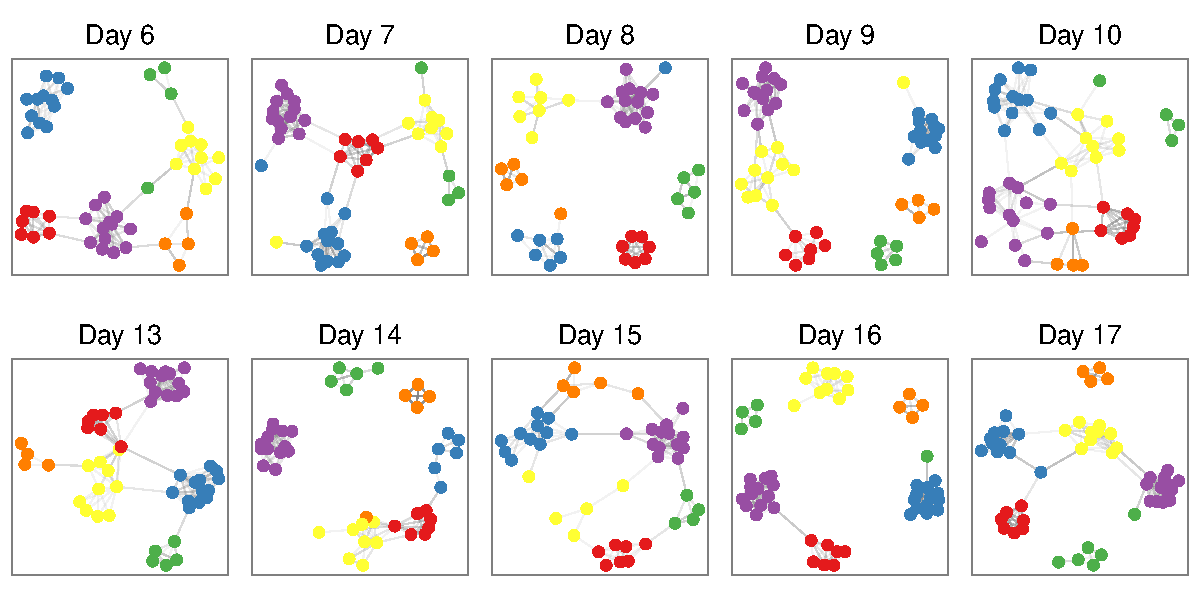
\includegraphics[width=\textwidth]{figure/email_facet_ggnet2-1.pdf}
\end{subfigure}

\begin{subfigure}[t]{\textwidth}
\caption{geomnet}
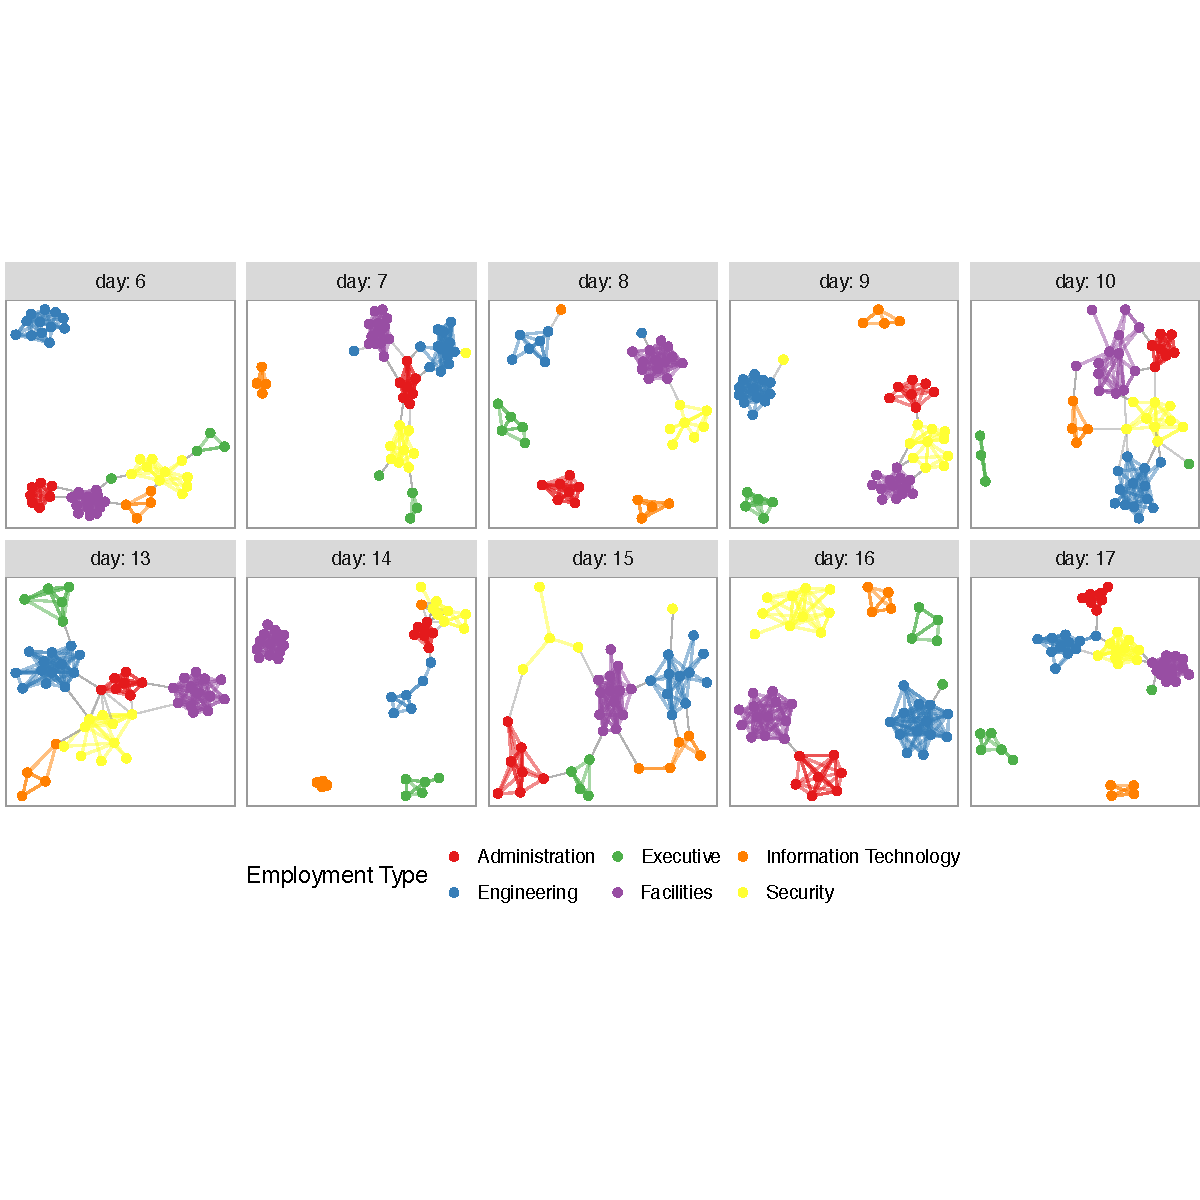
\includegraphics[width=\textwidth]{figure/email_facet_geom_net-1.pdf}
\end{subfigure}

\begin{subfigure}[t]{\textwidth}
\caption{ggnetwork}
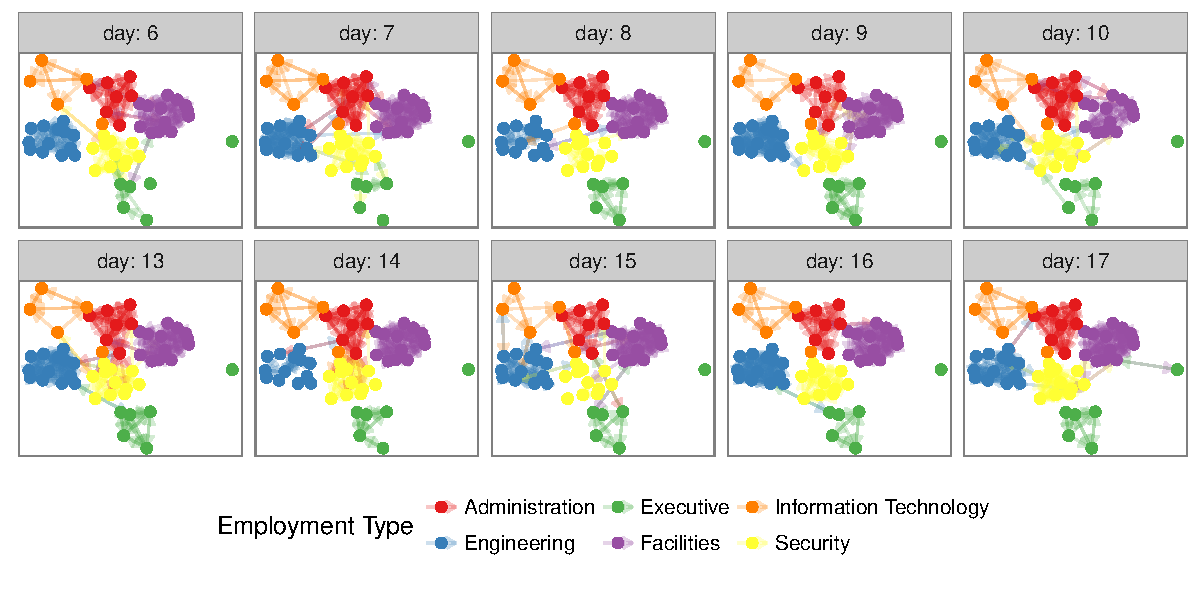
\includegraphics[width=\textwidth]{figure/email_facet_ggnetwork-1.pdf}
\end{subfigure}

\caption{\label{fig:email_facet} The same email network as in Figure~\ref{fig.cap:email} faceted by day of the week.}
\end{figure}
\afterpage{\clearpage}

\noindent
First, the code for the \code{ggnet2} approach, which results in Figure~\ref{fig:email_facet}(a):
\begin{knitrout}
\definecolor{shadecolor}{rgb}{1, 1, 1}\color{fgcolor}\begin{kframe}
\begin{verbatim}
# data preparation. first, remove emails sent to all employees
em.day <- subset(email$edges, nrecipients < 54)[, c("From", "to", "day") ]
# for small multiples by day, create one element in a list per day 
# (10 days, 10 elements in the list em.day)
em.day <- lapply(unique(em.day$day),
                 function(x) subset(em.day, day == x)[, 1:2 ])
# make the list of edgelists a list of network objects for plotting with ggnet2
em.day <- lapply(em.day, network, directed = TRUE)
# create vertex (employee type) and network (day) attributes for each element in list
for (i in 1:length(em.day)) {
  em.day[[ i ]] %v% "curr_empl_type" <-
    em.cet[ network.vertex.names(em.day[[ i ]]) ]
  em.day[[ i ]] %n% "day" <- unique(email$edges$day)[ i ]
}

# plot ggnet2
# first, make an empty list containing slots for the 10 days (one plot per day)
g <- list(length(em.day))
set.seed(7042016)
# create a ggnet2 plot for each element in the list of networks
for (i in 1:length(em.day)) {
  g[[ i ]] <- ggnet2(em.day[[ i ]], size = 2, 
                     color = "curr_empl_type",
                     palette = "Set1", arrow.size = 0,
                     arrow.gap = 0.01, edge.alpha = 0.1,
                     legend.position = "none", 
                     mode = "kamadakawai") +
    ggtitle(paste("Day", em.day[[ i ]] %n% "day")) +
    theme(panel.border = element_rect(color = "grey50", fill = NA),
          aspect.ratio = 1)
}
# arrange all of the network plots into one plot window
gridExtra::grid.arrange(grobs = g, nrow = 2)
\end{verbatim}
\end{kframe}
\end{knitrout}
\noindent
Second, the code for the \pkg{geomnet} approach, which results in Figure~\ref{fig:email_facet}(b):
\begin{knitrout}
\definecolor{shadecolor}{rgb}{1, 1, 1}\color{fgcolor}\begin{kframe}
\begin{verbatim}
# data step: use the fortify.edgedf group argument to 
# combine the edge and node data and allow all nodes to 
# show up on all days. Also, remove emails sent to all  
# employees
emailnet <- fortify(as.edgedf(subset(email$edges, nrecipients < 54)), email$nodes, group = "day")

# creating the plot
set.seed(7042016)
ggplot(data = emailnet, aes(from_id = from, to_id = to_id)) +
  geom_net(layout.alg = "kamadakawai", singletons = FALSE,
    aes(colour = CurrentEmploymentType,
        group = CurrentEmploymentType,
        linewidth = 2 * (...samegroup.. / 8 + .125)),
        arrowsize = .5,
        directed = TRUE, fiteach = TRUE, ealpha = 0.5, size = 1.5, na.rm = FALSE) +
  scale_colour_brewer("Employment Type", palette = "Set1") +
  theme_net() +
  facet_wrap(~day, nrow = 2, labeller = "label_both") +
  theme(legend.position = "bottom",
        panel.border = element_rect(fill = NA, colour = "grey60"),
        plot.margin = unit(c(0, 0, 0, 0), "mm"))
\end{verbatim}
\end{kframe}
\end{knitrout}

\noindent
Finally, the code for the \pkg{ggnetwork} approach, which results in Figure~\ref{fig:email_facet}(c):
\begin{knitrout}
\definecolor{shadecolor}{rgb}{1, 1, 1}\color{fgcolor}\begin{kframe}
\begin{verbatim}
# create the network and aesthetics
# first, remove emails sent to all employees
edges <- subset(email$edges, nrecipients < 54)
edges <- edges[, c("From", "to", "day") ]
# Create network class object for plotting with ggnetwork
em.net <- network(edges[, 1:2])
# assign edge attributes (day)
set.edge.attribute(em.net, "day", edges[, 3])
# assign vertex attributes (employee type)
em.net %v% "curr_empl_type" <- em.cet[ network.vertex.names(em.net) ]

# create the plot
set.seed(7042016)
ggplot(ggnetwork(em.net, arrow.gap = 0.02, by = "day", 
                 layout = "kamadakawai"),
       aes(x, y, xend = xend, yend = yend)) +
  geom_edges(
    aes(color = curr_empl_type),
    alpha = 0.25,
    arrow = arrow(length = unit(5, "pt"), type = "closed")) +
  geom_nodes(aes(color = curr_empl_type), size = 1.5) +
  scale_color_brewer("Employment Type", palette = "Set1") +
  facet_wrap(~day, nrow = 2, labeller = "label_both") +
  theme_facet(legend.position = "bottom")
\end{verbatim}
\end{kframe}
\end{knitrout}

Note the two key differences in the visualizations of Figure~\ref{fig:email_facet}: whether singletons (isolated nodes) are plotted (as in the \pkg{ggnetwork} method), and whether \emph{one} layout is used across all panels (as for the \code{ggnetwork} example) or whether individual layouts are fit to each of the subsets (as for the \code{ggnet2} and the \code{geomnet} examples). Plotting isolated nodes in \pkg{geomnet} is possible by setting \code{singletons = TRUE}, and it would be possible in \code{ggnet2} by including all nodes in the creation of the list of networks. Using the same layout for plotting small multiples in \code{geomnet} is controlled by the argument \code{fiteach}. By default, \code{fiteach = TRUE}, but \code{fiteach = FALSE} results in all panels sharing the same layout. Having the same layout in each panel makes seeing specific differences in ties between nodes easier, while having a different layout in each panel emphasizes the overall structural differences between the sub-networks. It would be interesting to be able to have a hybrid of these two approaches, but at the moment this is beyond the capability of any of the methods.
Through the faceting it becomes obvious that there are several days where one or more of the departments does not communicate with any of the other departments. There are only two days, day 13 and day 15, without any isolated department communications. Faceting is one of the major benefits of implementing tools for network visualization in \pkg{ggplot2}. Faceting allows the user to quickly separate dense networks into smaller sub-networks for easy visual comparison and analyses, a feature that the other network visualization tools do not have.

\subsection{\pkg{ggplot2} theme elements}

This example comes from the \code{theme()} help page in the \pkg{ggplot2} documentation \citep{ggplot2}.  It is a directed network which shows the structure of the inheritance of theme options in the construction of a \pkg{ggplot2} plot. There are 53 vertices and 36 edges in this network. Each vertex represents one possible theme option. There is an arrow from one theme option to another if the element represented by the `to' vertex inherits its values from the `from' vertex.  For example, the \code{axis.ticks.x} option inherits its value from the \code{axis.ticks} value, which in turn inherits its value from the \code{line} option.  Thus, setting the \code{line} option to a value such as \code{element\_blank()} sets the entire inheritance tree to \code{element\_blank()}, and no lines appear anywhere on the plot background.

\begin{figure}[hbtp]
\begin{subfigure}[t]{\textwidth}
\caption{ggnet2}
\vspace{1em}

             \begin{adjustbox}{valign=t}

             \begin{minipage}{.49\textwidth}
 \begin{knitrout}\footnotesize
\definecolor{shadecolor}{rgb}{1, 1, 1}\color{fgcolor}\begin{kframe}
\begin{verbatim}
# make data accessible
data(theme_elements, package = "geomnet")

# create network object
te.net <- network(theme_elements$edges)
# assign node attribut (size based on node degree)
te.net %v% "size" <-
  sqrt(10 * (sna::degree(te.net) + 1))
set.seed(3272016)
ggnet2(te.net, label = TRUE, color = "white", 
       label.size = "size", layout.exp = 0.15,
       mode = "fruchtermanreingold")
\end{verbatim}
\end{kframe}
\end{knitrout} \vspace{1em}

                   \end{minipage}

                  \begin{minipage}{.49\textwidth}

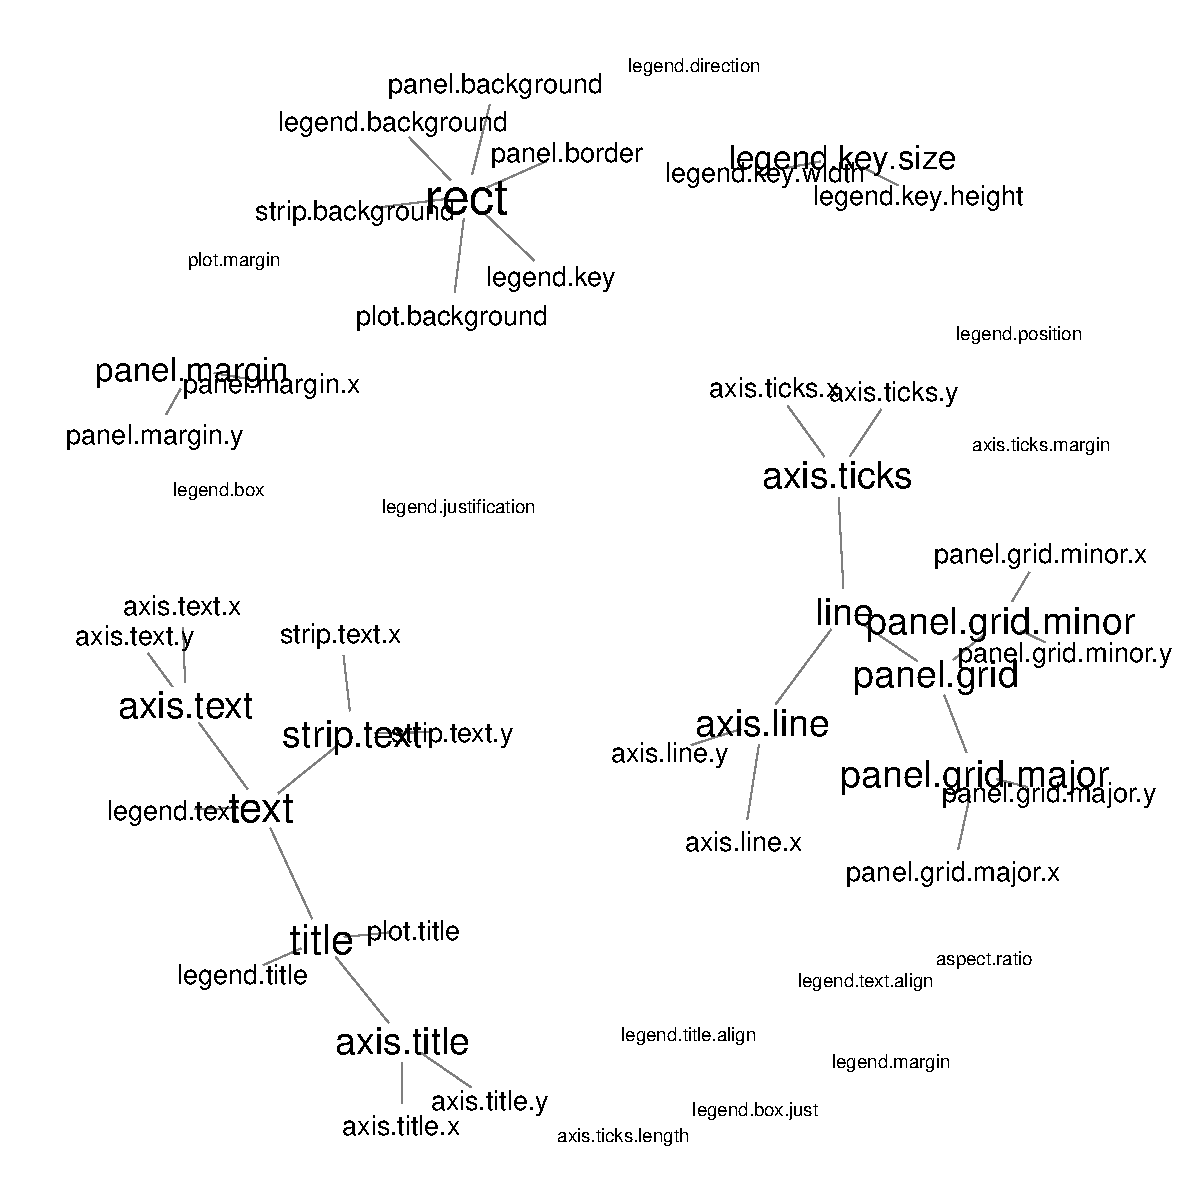
\includegraphics[width=\textwidth]{figure/theme_ggnet2-1.pdf}

                          \end{minipage}

                          \end{adjustbox}
\end{subfigure}

\begin{subfigure}[t]{\textwidth}
\caption{geomnet}
\vspace{1em}

             \begin{adjustbox}{valign=t}

             \begin{minipage}{.49\textwidth}
 \begin{knitrout}\footnotesize
\definecolor{shadecolor}{rgb}{1, 1, 1}\color{fgcolor}\begin{kframe}
\begin{verbatim}
# data step: merge nodes and edges and
# introduce a degree-out variable
# data step: merge nodes and edges and
# introduce a degree-out variable
TEnet <- fortify(
  as.edgedf(theme_elements$edges[,c(2,1)]),
            theme_elements$vertices)
TEnet <- TEnet %>%
  group_by(from_id) %>%
  mutate(degree = sqrt(10 * n() + 1))

# create plot:
set.seed(3272016)
ggplot(data = TEnet,
       aes(from_id = from_id, to_id = to_id)) +
  geom_net(layout.alg = "fruchtermanreingold",
    aes(fontsize = degree), directed = TRUE,
    labelon = TRUE, size = 1, labelcolour = 'black',
    ecolour = "grey70", arrowsize = 0.5,
    linewidth = 0.5, repel = TRUE) +
  theme_net() +
  xlim(c(-0.05, 1.05))
\end{verbatim}
\end{kframe}
\end{knitrout} \vspace{1em}

                   \end{minipage}

                  \begin{minipage}{.49\textwidth}

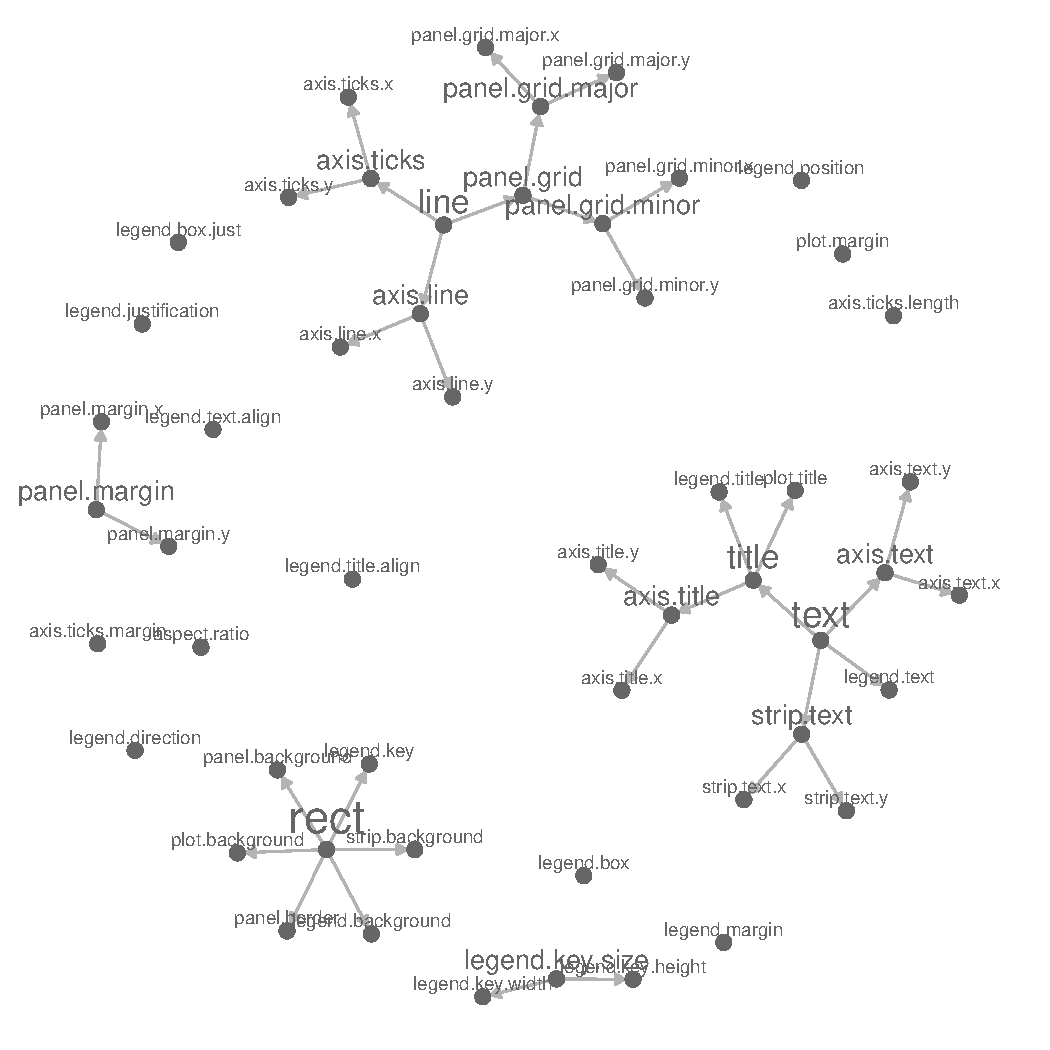
\includegraphics[width=\textwidth]{figure/theme_geom_net-1.pdf}

                          \end{minipage}

                          \end{adjustbox}
\end{subfigure}

\caption{\label{fig.cap:theme} Inheritance structure of \pkg{ggplot2} theme elements. This is a recreation of the graph found at \protect\url{http://docs.ggplot2.org/current/theme.html}.}
\end{figure}

\begin{figure}
\ContinuedFloat
\begin{subfigure}[t]{\textwidth}
\caption{ggnet2}
\vspace{1em}

             \begin{adjustbox}{valign=t}

             \begin{minipage}{.49\textwidth}
 \begin{knitrout}\footnotesize
\definecolor{shadecolor}{rgb}{1, 1, 1}\color{fgcolor}\begin{kframe}
\begin{verbatim}
set.seed(3272016)
# use network created in ggnet2 data step
ggplot(ggnetwork(te.net, 
                 layout = "fruchtermanreingold"),
       aes(x, y, xend = xend, yend = yend)) +
  geom_edges() +
  geom_nodes(size = 12, color = "white") +
  geom_nodetext(
    aes(size = size, label = vertex.names)) +
  scale_size_continuous(range = c(4, 8)) +
  guides(size = FALSE) +
  theme_blank()
\end{verbatim}
\end{kframe}
\end{knitrout} \vspace{1em}

                   \end{minipage}

                  \begin{minipage}{.49\textwidth}

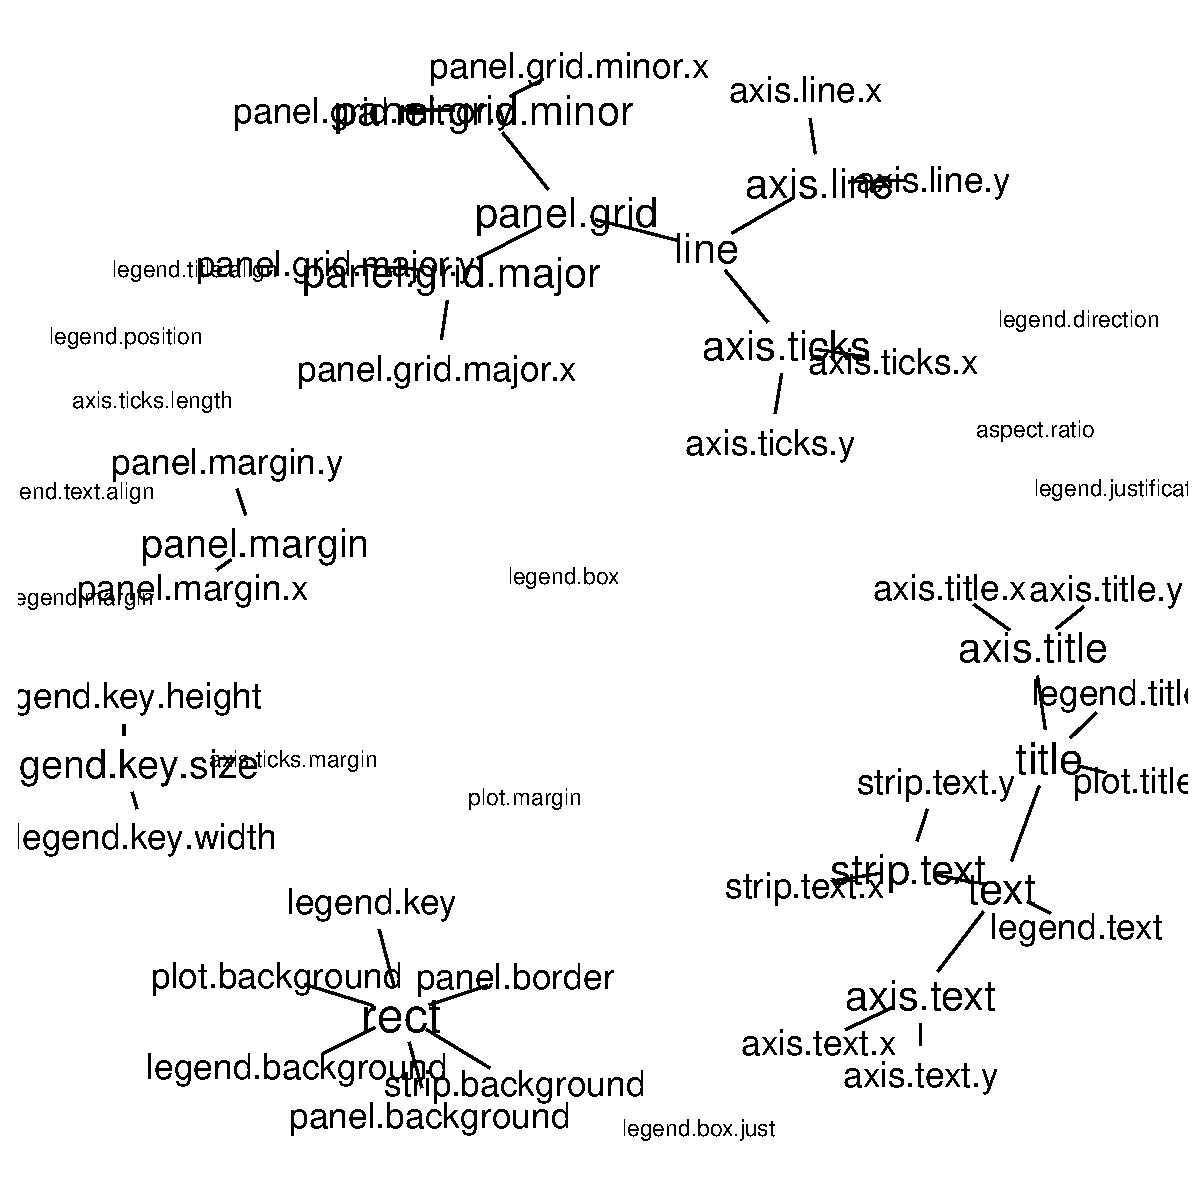
\includegraphics[width=\textwidth]{figure/theme_ggnetwork-1.pdf}

                          \end{minipage}

                          \end{adjustbox}
\end{subfigure}
\caption{\label{fig.cap:theme:c}(continued) Inheritance structure of \pkg{ggplot2} theme elements. This is a recreation of the graph found at \protect\url{http://docs.ggplot2.org/current/theme.html}.}
\end{figure}

\noindent
Code and plots of the inheritance structure are shown in Figure \ref{fig.cap:theme}. A glimpse of the data is below. 
\begin{knitrout}
\definecolor{shadecolor}{rgb}{1, 1, 1}\color{fgcolor}\begin{kframe}
\begin{verbatim}
te.net
##  Network attributes:
##   vertices = 53 
##   directed = TRUE 
##   hyper = FALSE 
##   loops = FALSE 
##   multiple = FALSE 
##   bipartite = FALSE 
##   total edges= 48 
##     missing edges= 0 
##     non-missing edges= 48 
## 
##  Vertex attribute names: 
##     size vertex.names 
## 
## No edge attributes
head(TEnet)
## Source: local data frame [6 x 3]
## Groups: from_id [2]
## 
##   from_id       to_id   degree
##    <fctr>      <fctr>    <dbl>
## 1    text       title 6.403124
## 2    text legend.text 6.403124
## 3    text   axis.text 6.403124
## 4    text  strip.text 6.403124
## 5    line   axis.line 5.567764
## 6    line  axis.ticks 5.567764
\end{verbatim}
\end{kframe}
\end{knitrout}
Note the various ways the packages adjust the side of the labels to correspond to the outdegree of the nodes, including the use of the \code{scale\_size\_continuous} function in Figure \ref{fig.cap:theme}(c). In each of these plots, it is easy to quickly determine  parent-child relationships, and to assess which theme elements are unrelated to all others. Nodes with the most children are the \code{rect}, \code{text}, and \code{line} elements, so we made their labels larger in order to emphasize their importance. In each case, the label size is a function of the out degree of the vertices.

\subsection{College football}

This next example comes from M.E.J. Newman's network data web page \citep{football}.  It is an undirected network consisting of all regular season college football games played between Division I schools in Fall of 2000.  There are 115 vertices and 613 edges: each vertex represents a school, and an edge represents a game played between two schools. There is an additional variable in the vertex data frame corresponding to the conference each team belongs to, and there is an additional variable in the edge data frame that is equal to one if the game occurred between teams in the same conference or zero if the game occurred between teams in different conferences. We take a look at the data used in the plots below.


  
\begin{knitrout}
\definecolor{shadecolor}{rgb}{1, 1, 1}\color{fgcolor}\begin{kframe}
\begin{verbatim}
fb.net 
##  Network attributes:
##   vertices = 115 
##   directed = TRUE 
##   hyper = FALSE 
##   loops = FALSE 
##   multiple = FALSE 
##   bipartite = FALSE 
##   total edges= 613 
##     missing edges= 0 
##     non-missing edges= 613 
## 
##  Vertex attribute names: 
##     conf vertex.names 
## 
##  Edge attribute names: 
##     same.conf
head(ftnet)
##    from_id             to_id same.conf         value
## 1 AirForce    NevadaLasVegas         1 Mountain West
## 2    Akron         MiamiOhio         1  Mid-American
## 3    Akron      VirginiaTech         0  Mid-American
## 4    Akron           Buffalo         1  Mid-American
## 5    Akron BowlingGreenState         1  Mid-American
## 6    Akron              Kent         1  Mid-American
##   schools
## 1        
## 2        
## 3        
## 4        
## 5        
## 6
\end{verbatim}
\end{kframe}
\end{knitrout}

The network of football games is given in Figure~\ref{fig.cap:football}. Here,  the \code{linetype} aesthetic  corresponds to games that occur between teams in the same conference or different conferences.  

\begin{figure}[hbtp]
\begin{subfigure}[t]{\textwidth}
\caption{ggnet2}\vspace{-.5cm}
\vspace{1em}

             \begin{adjustbox}{valign=t}

             \begin{minipage}{.49\textwidth}
 \begin{knitrout}\footnotesize
\definecolor{shadecolor}{rgb}{1, 1, 1}\color{fgcolor}\begin{kframe}
\begin{verbatim}
#make data accessible
data(football, package = 'geomnet')
rownames(football$vertices) <-
  football$vertices$label
# create network 
fb.net <- network(football$edges[, 1:2],
                  directed = TRUE)
# create node attribute 
# (what conference is team in?)
fb.net %v% "conf" <-
  football$vertices[
    network.vertex.names(fb.net), "value"
    ]
# create edge attribute 
# (between teams in same conference?)
set.edge.attribute(
  fb.net, "same.conf",
  football$edges$same.conf)
set.seed(5232011)
ggnet2(fb.net, mode = "fruchtermanreingold",
       color = "conf",  palette = "Paired",
       color.legend = "Conference",
       edge.color = c("color", "grey75"))
\end{verbatim}
\end{kframe}
\end{knitrout} \vspace{1em}

                   \end{minipage}

                  \begin{minipage}{.49\textwidth}

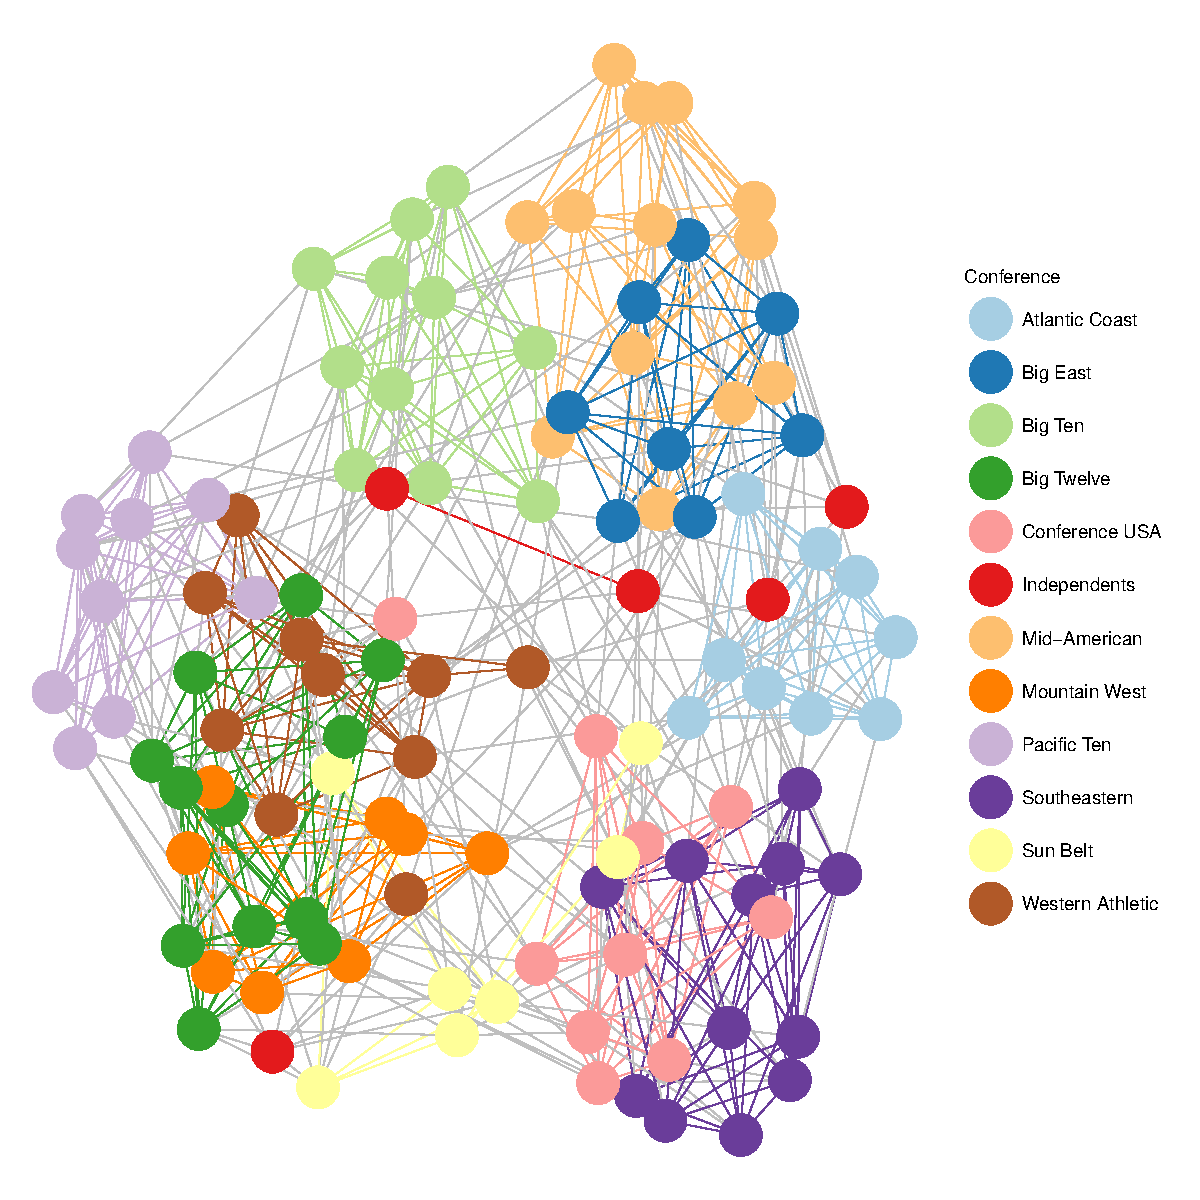
\includegraphics[width=\textwidth]{figure/football_ggnet2-1.pdf}

                          \end{minipage}

                          \end{adjustbox}
\end{subfigure}

\end{figure}

\begin{figure}
\ContinuedFloat
\begin{subfigure}[t]{\textwidth}
\caption{geomnet}\vspace{-.5cm}
\vspace{1em}

             \begin{adjustbox}{valign=t}

             \begin{minipage}{.49\textwidth}
 \begin{knitrout}\footnotesize
\definecolor{shadecolor}{rgb}{1, 1, 1}\color{fgcolor}\begin{kframe}
\begin{verbatim}
# data step: merge vertices and edges
# data step: merge vertices and edges
ftnet <- fortify(as.edgedf(football$edges), 
                 football$vertices)

# create new label variable for independent schools
ftnet$schools <- ifelse(
  ftnet$value == "Independents", ftnet$from_id, "")

# create data plot
set.seed(5232011)
ggplot(data = ftnet,
       aes(from_id = from_id, to_id = to_id)) +
  geom_net(layout.alg = 'fruchtermanreingold',
    aes(colour = value, group = value,
        linetype = factor(same.conf != 1),
        label = schools),
    linewidth = 0.5,
    size = 5, vjust = -0.75, alpha = 0.3) +
  theme_net() +
  theme(legend.position = "bottom") +
  scale_colour_brewer("Conference", palette = "Paired")  +
  guides(linetype = FALSE)
\end{verbatim}
\end{kframe}
\end{knitrout} \vspace{1em}

                   \end{minipage}

                  \begin{minipage}{.49\textwidth}

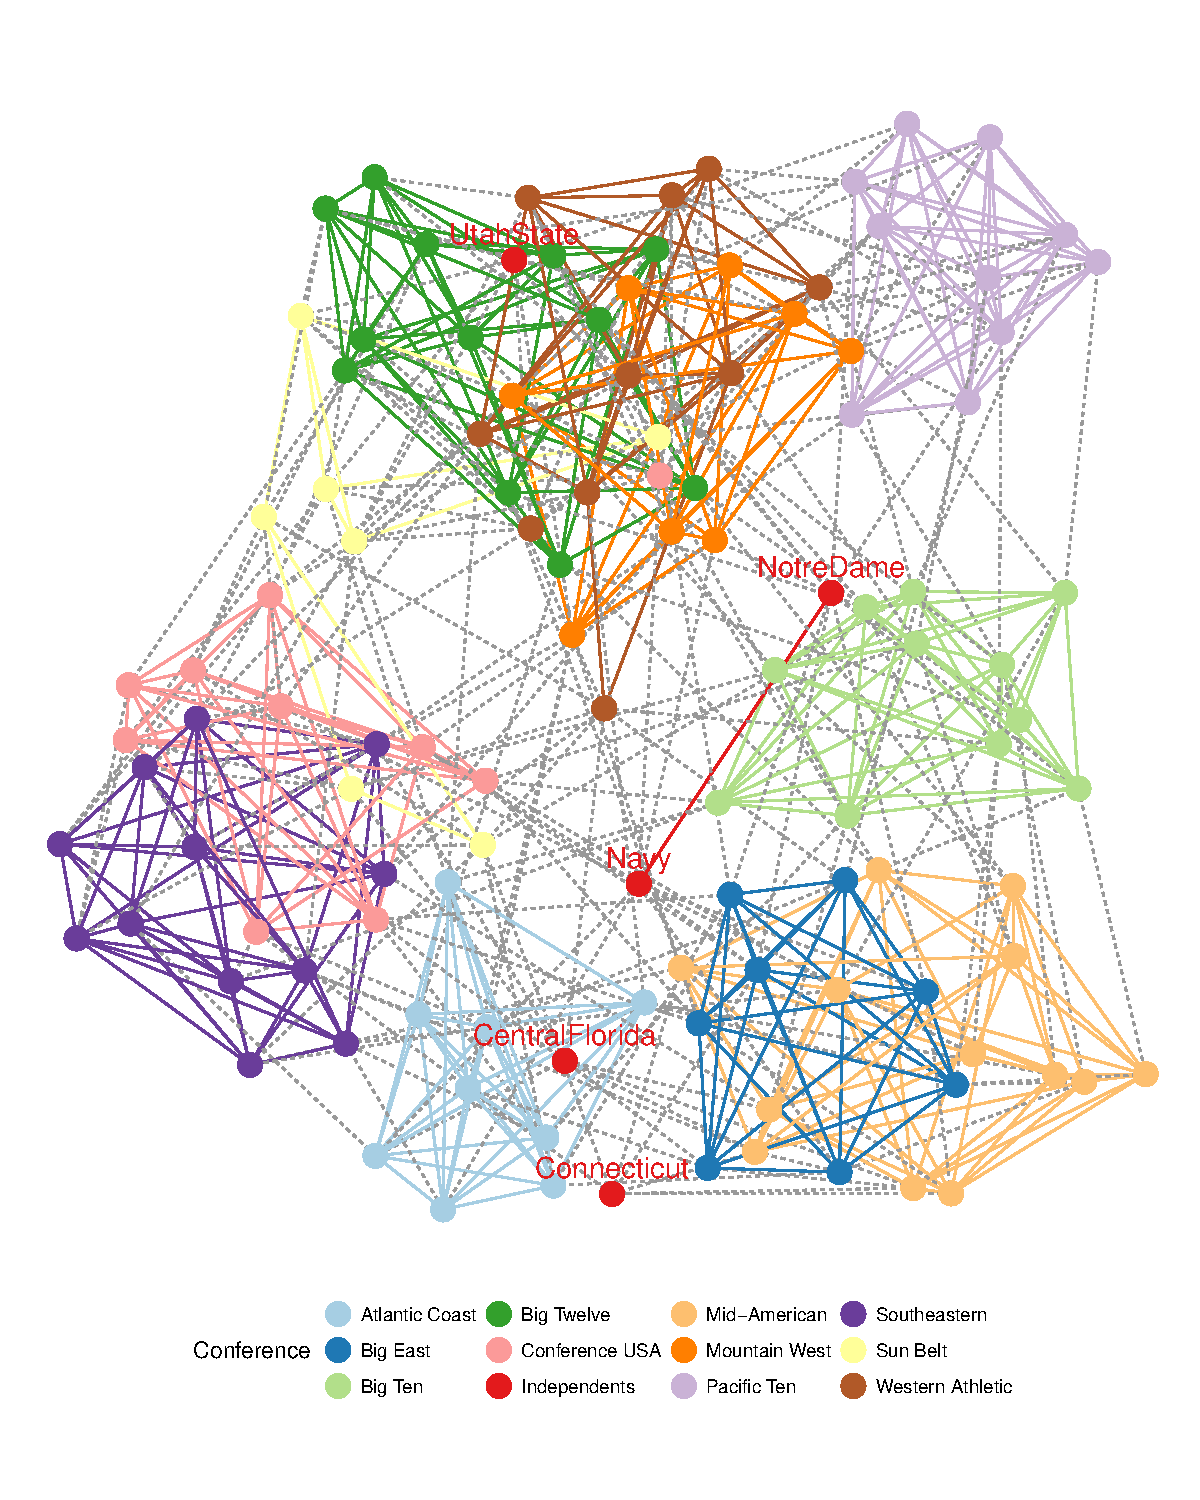
\includegraphics[width=\textwidth]{figure/football_geom_net-1.pdf}

                          \end{minipage}

                          \end{adjustbox}
\end{subfigure}

\begin{subfigure}[t]{\textwidth}
\caption{ggnetwork}\vspace{-.5cm}

\vspace{1em}

             \begin{adjustbox}{valign=t}

             \begin{minipage}{.49\textwidth}
 \begin{knitrout}\footnotesize
\definecolor{shadecolor}{rgb}{1, 1, 1}\color{fgcolor}\begin{kframe}
\begin{verbatim}
# use network from ggnet2 step
set.seed(5232011)
ggplot(
  ggnetwork(
    fb.net, 
    layout = "fruchtermanreingold"),
  aes(x, y, xend = xend, yend = yend)) +
  geom_edges(
    aes(linetype = as.factor(same.conf)),
    color = "grey50") +
  geom_nodes(aes(color = conf), size = 4) +
  scale_color_brewer("Conference",
                     palette = "Paired") +
  scale_linetype_manual(values = c(2,1)) +
  guides(linetype = FALSE) +
  theme_blank()
\end{verbatim}
\end{kframe}
\end{knitrout} \vspace{1em}

                   \end{minipage}

                  \begin{minipage}{.49\textwidth}

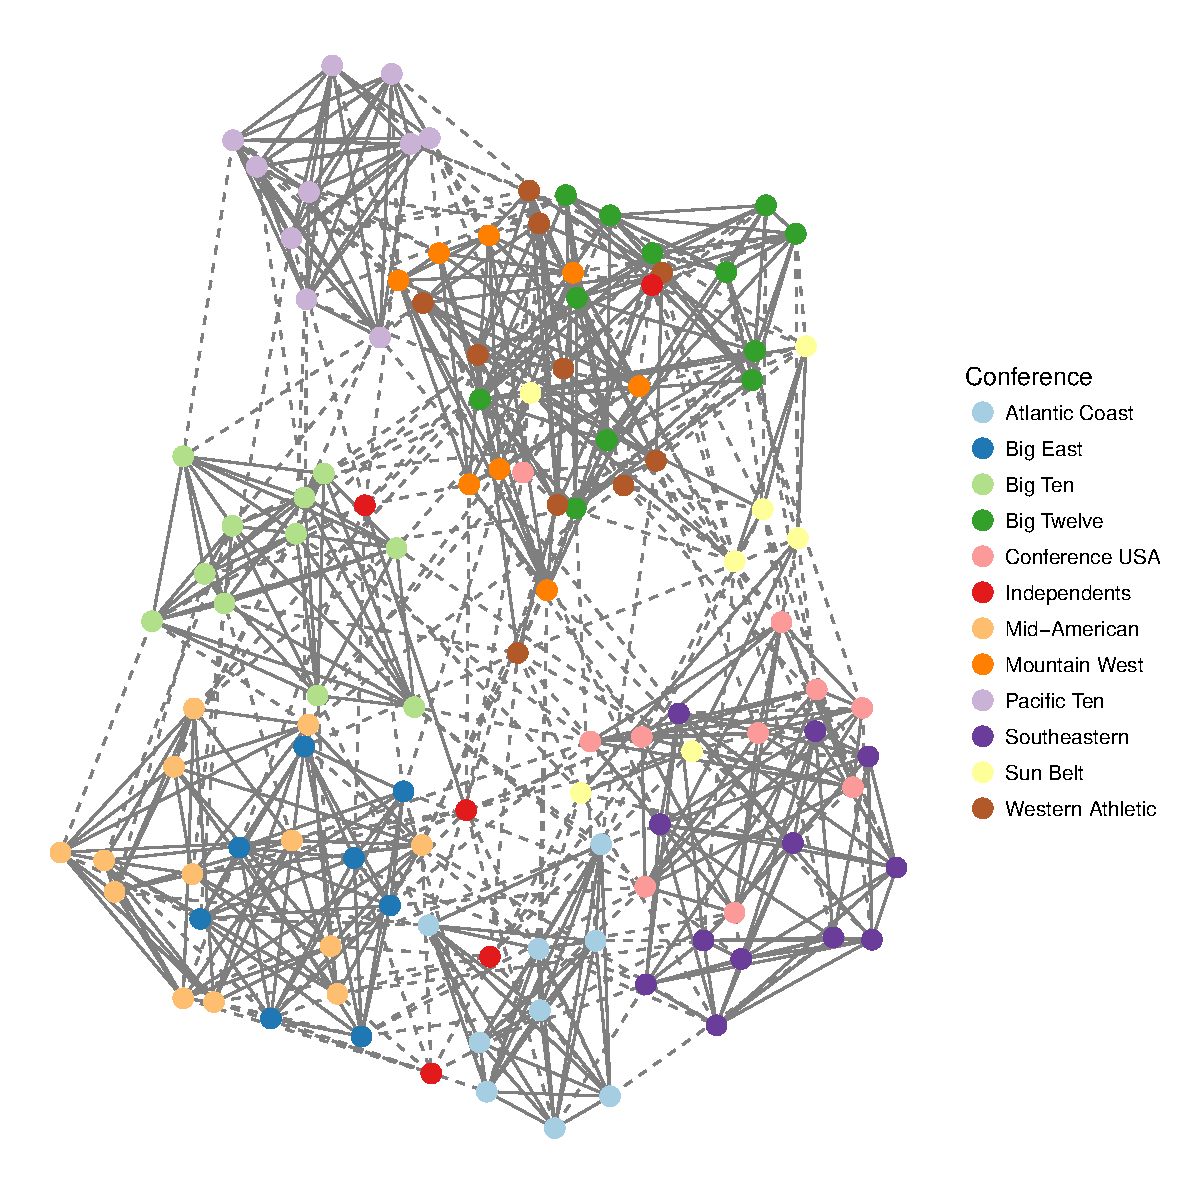
\includegraphics[width=\textwidth]{figure/football_ggnetwork-1.pdf}

                          \end{minipage}

                          \end{adjustbox}
\end{subfigure}
\caption{\label{fig.cap:football}(continued) The network of regular season Division I college football games in the season of fall 2000. The vertices and their labels are colored by conference.}
\end{figure}

\noindent
These lines are dotted and solid, respectively. We have also assigned a different color to each conference, so that the vertices and their labels are colored according to their conference. Additionally, in the first two implementations, the edges between two teams in the same conference share that conference color, while edges between teams in different conferences are a default gray color. This coloring and changing of the line types make the structure of the game network easier to view. Additionally, we use the \code{label} aesthetic in Figure \ref{fig.cap:football}(b) to label only a few schools that are of interest to us. This is the conference consisting of Navy, Notre Dame, Utah State, Central Florida, and Connecticut, which is spread out, whereas most other conferences' teams are all very close to each other because they play within conference much more than they play out of conference.  At the time, these five schools were all independents and did not have a home conference.  Without the coloring capability, we would not have been able to pick out that difference as easily.

\subsection{Southern women} 

Bipartite (or `two-mode') networks are networks with two different kinds of nodes and where all ties are formed between these two kinds. Affiliation networks, which represent the ties between individuals and the groups to which they belong, are examples of such networks \citep[see][p.~53-54 and p.~123-127]{newman}.

One of the classic examples for a two-mode network is the network of 18 Southern women attending 14 social events as collected by \citet{davis} and published e.g.\ as part of the \CRANpkg{tnet} package \citep{tnet}. In this data, a woman is linked by an edge to an event if she attended it. 
One of the questions for these type of networks is gain insight in the interplay between the two different sets of nodes. 

The data for the example of the Southern women is reported as edge list in form of `lady $X$ attending event $Y$'.
With a bit of data preparation as detailed below, we can visualize the graph as shown in Figure~\ref{fig:davis}. In creating the plots, we use the \code{shape} and \code{colour} aesthetics to map the two different modes to two different shapes and colours. 

\begin{knitrout}
\definecolor{shadecolor}{rgb}{1, 1, 1}\color{fgcolor}\begin{kframe}
\begin{verbatim}
# access the data and rename it for convenience
library(tnet)

data(tnet)
elist <- data.frame(Davis.Southern.women.2mode)
names(elist) <- c("Lady", "Event")
\end{verbatim}
\end{kframe}
\end{knitrout}

\noindent
The edge list for the Southern women's data consists of women attending events:
\begin{knitrout}
\definecolor{shadecolor}{rgb}{1, 1, 1}\color{fgcolor}\begin{kframe}
\begin{verbatim}
head(elist,4)
##   Lady Event
## 1    1     1
## 2    1     2
## 3    1     3
## 4    1     4
\end{verbatim}
\end{kframe}
\end{knitrout}
\noindent
In order to distinguish between nodes from different types, we have to add an additional identifier element, so that we can tell the `first' woman $L1$ apart from the first event, $E1$.
\begin{knitrout}
\definecolor{shadecolor}{rgb}{1, 1, 1}\color{fgcolor}\begin{kframe}
\begin{verbatim}
elist$Lady <- paste("L", elist$Lady, sep="")
elist$Event <- paste("E", elist$Event, sep="")

davis <- elist
names(davis) <- c("from", "to")
davis <- rbind(davis, data.frame(from=davis$to, to=davis$from))
davis$type <- factor(c(rep("Lady", nrow(elist)), rep("Event", nrow(elist))))
\end{verbatim}
\end{kframe}
\end{knitrout}

\begin{figure}[bh]
\begin{subfigure}[t]{\textwidth}
\caption{\code{ggnet2}}
\vspace{1em}

             \begin{adjustbox}{valign=t}

             \begin{minipage}{.49\textwidth}
 \begin{knitrout}\footnotesize
\definecolor{shadecolor}{rgb}{1, 1, 1}\color{fgcolor}\begin{kframe}
\begin{verbatim}
# Southern women network in ggnet2
# create affiliation matrix
bip = xtabs(~Event+Lady, data=elist)

# weighted bipartite network
bip = network(bip,
              matrix.type = "bipartite",
              ignore.eval = FALSE,
              names.eval = "weights")

# detect and color the mode
set.seed(8262013)
ggnet2(bip, color = "mode", palette = "Set2", 
       shape = "mode", mode = "kamadakawai",
       size = 15, label = TRUE) +
  theme(legend.position="bottom")
\end{verbatim}
\end{kframe}
\end{knitrout} \vspace{1em}

                   \end{minipage}

                  \begin{minipage}{.49\textwidth}

\includegraphics[width=\textwidth]{figure/davis_ggnet2-1.pdf}

                          \end{minipage}

                          \end{adjustbox}
\end{subfigure}
\caption{Graph of the Southern women data. Women are represented as orange triangles, events as green circles. }
\end{figure}
\begin{figure}
\ContinuedFloat
\begin{subfigure}[t]{\textwidth}
\caption{\pkg{geomnet}}
\vspace{1em}

             \begin{adjustbox}{valign=t}

             \begin{minipage}{.49\textwidth}
 \begin{knitrout}\footnotesize
\definecolor{shadecolor}{rgb}{1, 1, 1}\color{fgcolor}\begin{kframe}
\begin{verbatim}
# Southern women network in geomnet
# change labelcolour
davis$lcolour <- 
  c("white", "black")[as.numeric(davis$type)]

set.seed(8262013)
ggplot(data = davis) + 
  geom_net(layout.alg = "kamadakawai",
    aes(from_id = from, to_id = to, 
        colour = type, shape = type), 
    size = 15, labelon = TRUE, ealpha = 0.25,
    vjust = 0.5, hjust = 0.5,
    labelcolour = davis$lcolour) +
  theme_net() + 
  scale_colour_brewer("Type of node", palette = "Set2") +
  scale_shape("Type of node") +
  theme(legend.position = "bottom")
\end{verbatim}
\end{kframe}
\end{knitrout} \vspace{1em}

                   \end{minipage}

                  \begin{minipage}{.49\textwidth}

\includegraphics[width=\textwidth]{figure/davis_geom_net-1.pdf}

                          \end{minipage}

                          \end{adjustbox}
\end{subfigure}
\begin{subfigure}[t]{\textwidth}
\caption{\pkg{ggnetwork}}
\vspace{1em}

             \begin{adjustbox}{valign=t}

             \begin{minipage}{.49\textwidth}
 \begin{knitrout}\footnotesize
\definecolor{shadecolor}{rgb}{1, 1, 1}\color{fgcolor}\begin{kframe}
\begin{verbatim}
# Southern women network in ggnetwork. Use data from ggnet2 step
# assign vertex attributes (Node type and label)
set.vertex.attribute(bip, "mode", 
  c(rep("event", 14), rep("woman", 18)))
set.seed(8262013)
ggplot(data = ggnetwork(bip, 
        layout = "kamadakawai"),
    aes(x = x, y = y, xend = xend, yend = yend)) + 
  geom_edges(colour = "grey80") +
  geom_nodes(aes(colour = mode, shape = mode), 
             size = 15) +
  geom_nodetext(aes(label = vertex.names)) +
  scale_colour_brewer(palette = "Set2") +
  theme_blank() + 
  theme(legend.position = "bottom") 
\end{verbatim}
\end{kframe}
\end{knitrout} \vspace{1em}

                   \end{minipage}

                  \begin{minipage}{.49\textwidth}

\includegraphics[width=\textwidth]{figure/davis_ggnetwork-1.pdf}

                          \end{minipage}

                          \end{adjustbox}
\end{subfigure}
\caption{\label{fig:davis} Graph of the Southern women data. Women are represented as orange triangles, events as green circles. }
\end{figure}

\noindent The two different types of nodes are shown by different shapes and colors. We see the familiar relationship between events and groups of women attending these events. Women attending the same events then form a tighter knit subset, while events are also thought of as more similar, if they are attended by the same women. This defines the cluster of events E1 through E5, which are only attended by women 1 through 9, while events E6 through E9 are attended by (almost) everybody making them the core group of events.   


\subsection{Bike sharing in Washington D.C.} 
  
The data shows trips taken with bikes from the bike share company Capital Bikeshare\footnote{\url{https://secure.capitalbikeshare.com/}} during the second quarter of 2015. While this bike sharing company is located in the heart of Washington D.C.\ the company offers a set of bike stations just outside of Washington in Rockville, MD and north of it. Each station is shown as a vertex, and edges between stations indicate that at least five trips were taken between these two stations; the wider the line, the more trips have been taken between stations. In order to reflect distance between stations, we use as an additional restriction that the fastest trip was at most ten minutes long.
Figure~\ref{fig:bikes} shows four renderings of this data. The first is a geographically true representation of the area overlaid by lines between bike stations, the other three are networks drawn with \pkg{geomnet}, \code{ggnet2}, and \pkg{ggnetwork}, respectively. 
The code for these renderings is shown below:

\begin{knitrout}
\definecolor{shadecolor}{rgb}{1, 1, 1}\color{fgcolor}\begin{kframe}
\begin{verbatim}
# make data accessible
data(bikes, package = 'geomnet')
# data step for geomnet
tripnet <- fortify(as.edgedf(bikes$trips), bikes$stations[,c(2,1,3:5)])
# create variable to identify Metro Stations
tripnet$Metro = FALSE
idx <- grep("Metro", tripnet$from_id)
tripnet$Metro[idx] <- TRUE
\end{verbatim}
\end{kframe}
\end{knitrout}

\begin{knitrout}
\definecolor{shadecolor}{rgb}{1, 1, 1}\color{fgcolor}\begin{kframe}
\begin{verbatim}
# plot the bike sharing network shown in Figure 7b
set.seed(1232016)
ggplot(aes(from_id = from_id, to_id = to_id), data = tripnet) +
  geom_net(aes(linewidth = n / 15, colour = Metro),
           labelon = TRUE, repel = TRUE) +
  theme_net() +
  xlim(c(-0.1, 1.1)) +
  scale_colour_manual("Metro Station", values = c("grey40", "darkorange")) +
  theme(legend.position = "bottom")
\end{verbatim}
\end{kframe}
\end{knitrout}

\begin{knitrout}
\definecolor{shadecolor}{rgb}{1, 1, 1}\color{fgcolor}\begin{kframe}
\begin{verbatim}
# data preparation for ggnet2 and ggnetwork
bikes.net <- network(bikes$trips[, 1:2 ], directed = FALSE)
# create edge attribute (number of trips)
network::set.edge.attribute(bikes.net, "n", bikes$trips[, 3 ] / 15)
# create vertex attribute for Metro Station
bikes.net %v% "station" <-  grepl("Metro", network.vertex.names(bikes.net))
bikes.net %v% "station" <-  1 + as.integer(bikes.net %v% "station")
rownames(bikes$stations) <- bikes$stations$name
# create node attributes (coordinates)
bikes.net %v% "lon" <-
  bikes$stations[ network.vertex.names(bikes.net), "long" ]
bikes.net %v% "lat" <-
  bikes$stations[ network.vertex.names(bikes.net), "lat" ]
bikes.col <- c("grey40", "darkorange")
\end{verbatim}
\end{kframe}
\end{knitrout}
  
\begin{knitrout}
\definecolor{shadecolor}{rgb}{1, 1, 1}\color{fgcolor}\begin{kframe}
\begin{verbatim}
# Non-geographic placement
set.seed(1232016)
ggnet2(bikes.net, mode = "fruchtermanreingold", size = 4, label = TRUE,
       vjust = -0.5, edge.size = "n", layout.exp = 1.1,
       color = bikes.col[ bikes.net %v% "station" ],
       label.color = bikes.col[ bikes.net %v% "station" ])
\end{verbatim}
\end{kframe}
\end{knitrout}
  
\begin{knitrout}
\definecolor{shadecolor}{rgb}{1, 1, 1}\color{fgcolor}\begin{kframe}
\begin{verbatim}
# Non-geographic placement. Use data from ggnet2 step.
set.seed(1232016)
ggplot(data = ggnetwork(bikes.net, layout = "fruchtermanreingold"),
         aes(x, y, xend = xend, yend = yend)) +
  geom_edges(aes(size = n), color = "grey40") +
  geom_nodes(aes(color = factor(station)), size = 4) +
  geom_nodetext(aes(label = vertex.names, color = factor(station)),
                vjust = -0.5) +
  scale_size_continuous("Trips", breaks = c(2, 4, 6), labels = c(30, 60, 90)) +
  scale_colour_manual("Metro station", labels = c("FALSE", "TRUE"),
                      values = c("grey40", "darkorange")) +
  theme_blank() +
  theme(legend.position = "bottom", legend.box = "horizontal")
\end{verbatim}
\end{kframe}
\end{knitrout}
  

\begin{figure}[hbtp]
\begin{subfigure}[t]{.49\textwidth}
\caption{geographic map}
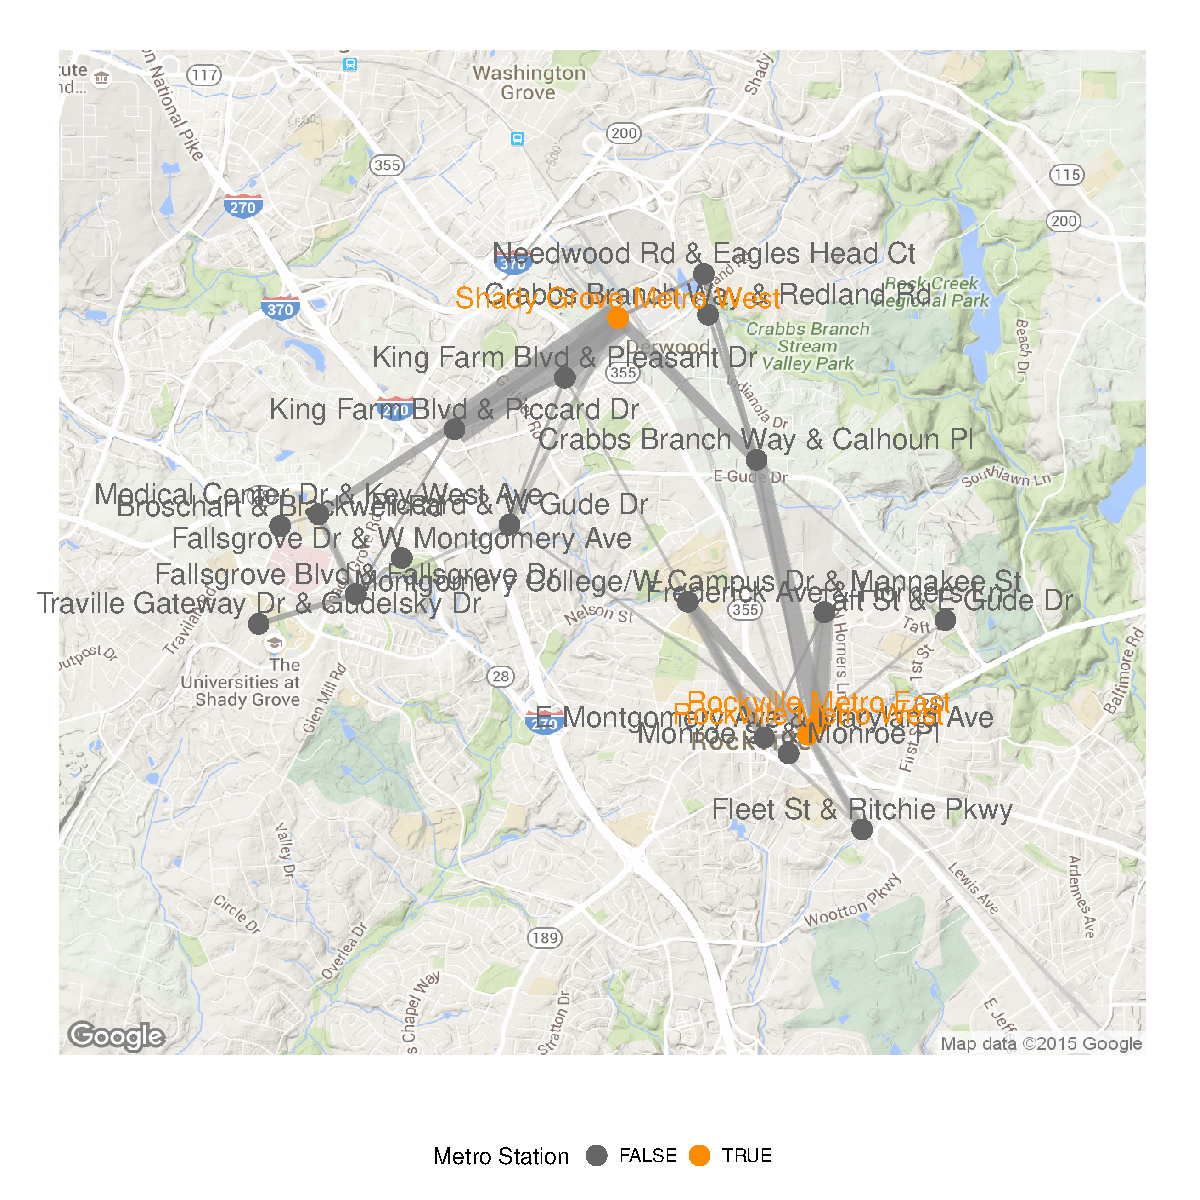
\includegraphics[width=\textwidth]{figure/geographic_geomnet-1.pdf}
\end{subfigure}
\begin{subfigure}[t]{.49\textwidth}
\caption{geomnet}
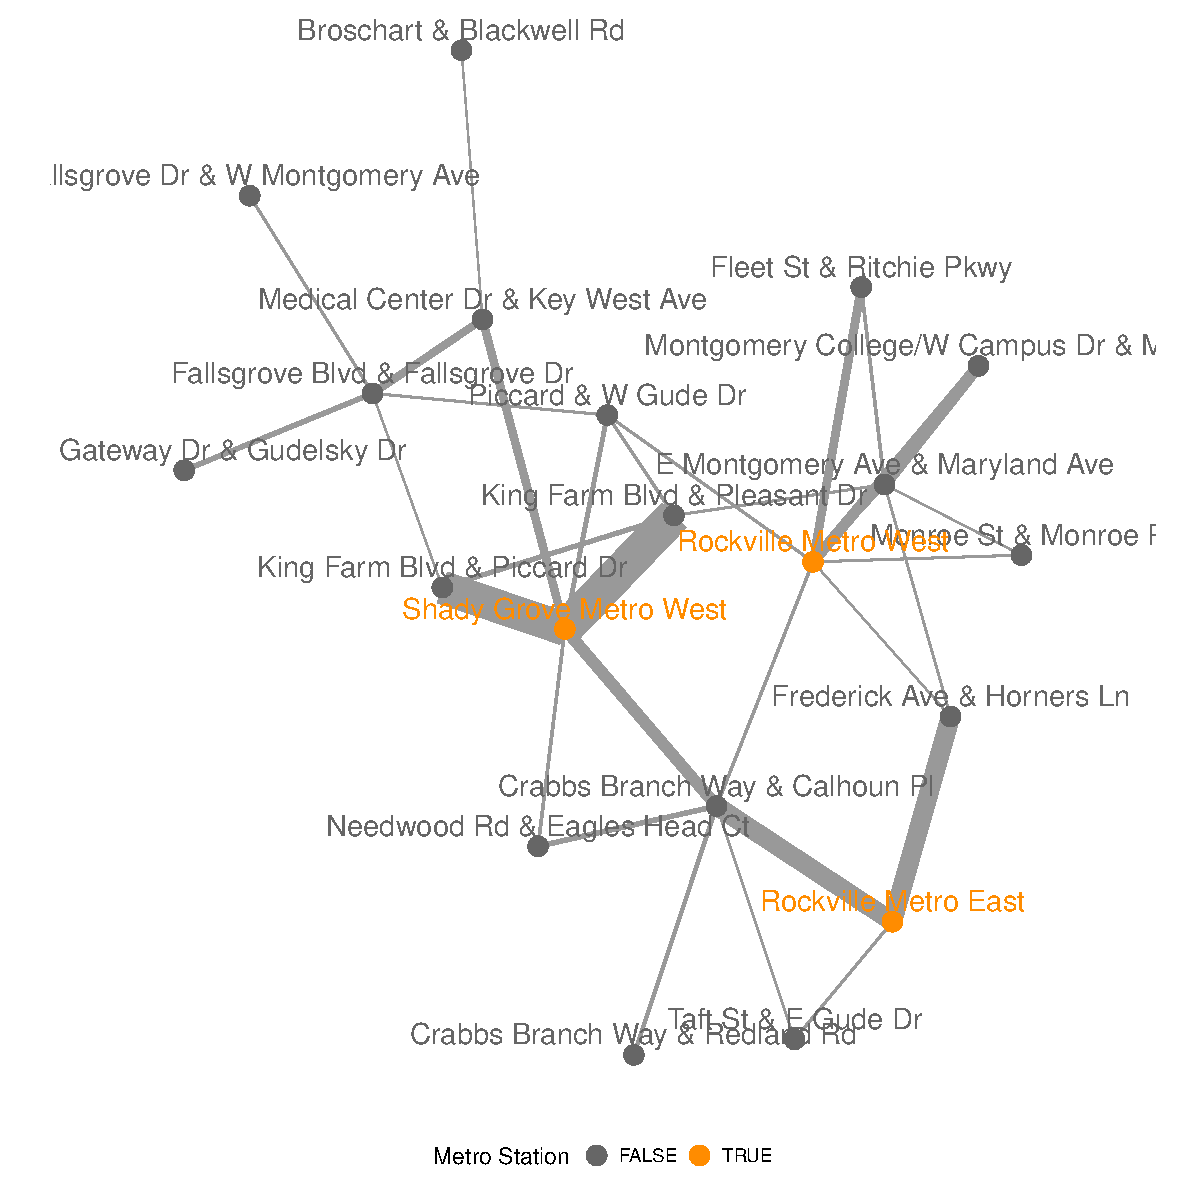
\includegraphics[width=\textwidth]{figure/bikes_geom_net-1.pdf}
\end{subfigure}
\begin{subfigure}[t]{.49\textwidth}
\caption{ggnet2}
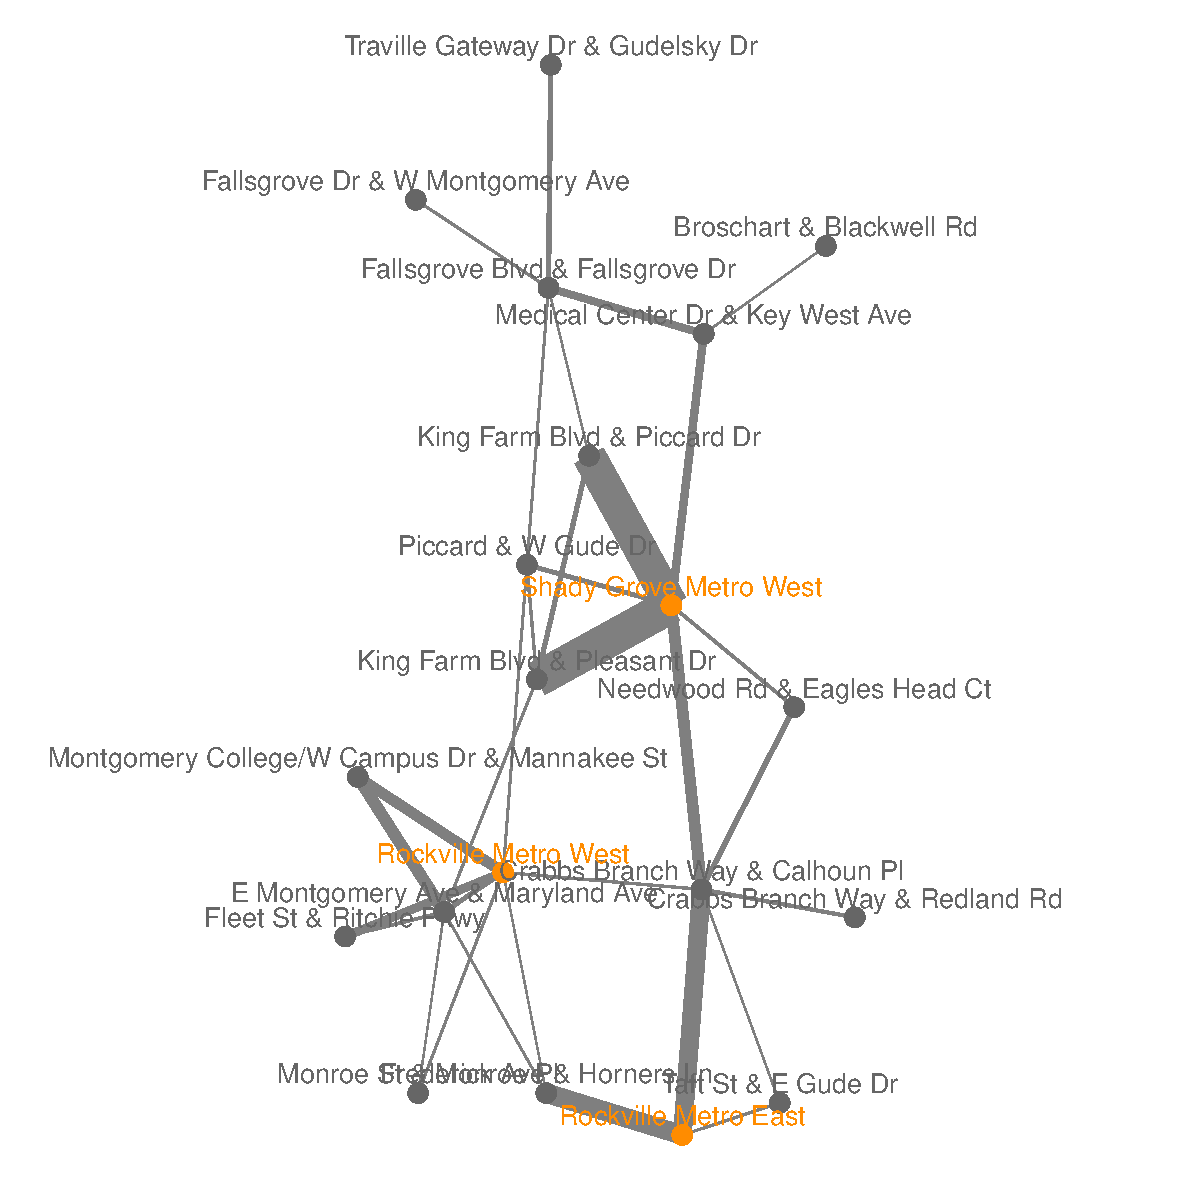
\includegraphics[width=\textwidth]{figure/bikes_ggnet2-1.pdf}
\end{subfigure}
\begin{subfigure}[t]{.49\textwidth}
\caption{ggnetwork}
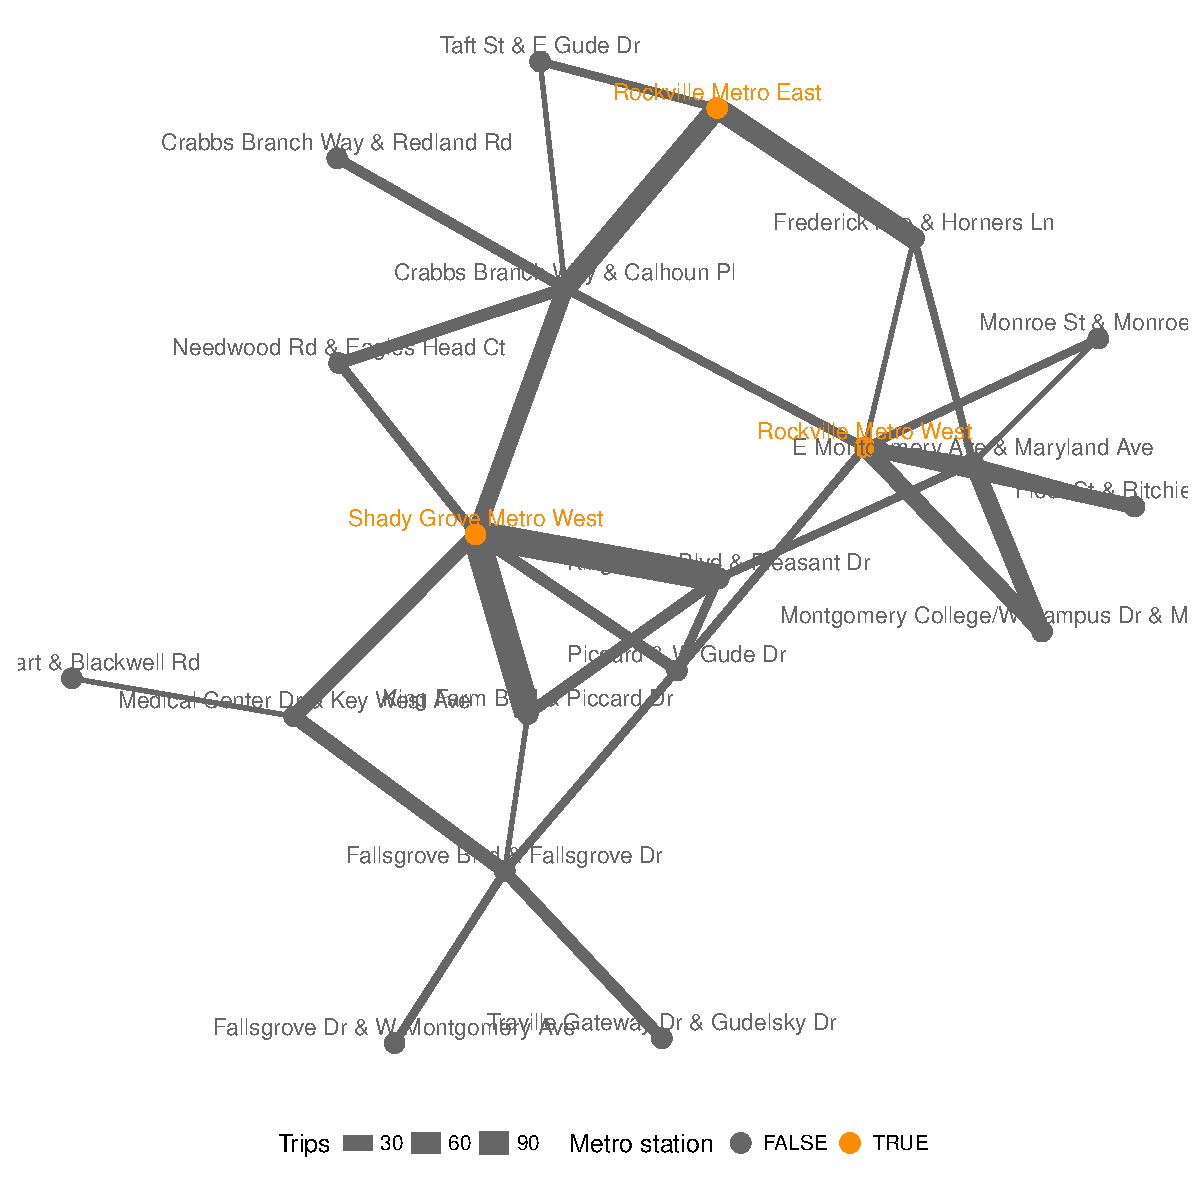
\includegraphics[width=\textwidth]{figure/bikes_ggnetwork-1.pdf}
\end{subfigure}
\caption{\label{fig:bikes}Network of bike trips using a geographically true representation(top left) overlaid on a satellite map, a Kamada-Kawai layout in \pkg{geomnet} (top right), a Fruchterman-Reingold layout in \code{ggnet2} (bottom left) and \pkg{ggnetwork} (bottom right). Metro stations are shown in orange. In both the Kamada-Kawai and the Fruchterman-Reingold layouts, metro stations take a much more central position than in the geographically true representation.}
\end{figure}

To plot the geographically correct bike network layout in \pkg{geomnet}, we use the \samp{layout.alg = NULL} option and provide the latitude and longitude coordinates of the bike stations from the company's data. A glance of the data that we used in the examples is shown below. 
\begin{knitrout}
\definecolor{shadecolor}{rgb}{1, 1, 1}\color{fgcolor}\begin{kframe}
\begin{verbatim}
bikes.net
##  Network attributes:
##   vertices = 20 
##   directed = FALSE 
##   hyper = FALSE 
##   loops = FALSE 
##   multiple = FALSE 
##   bipartite = FALSE 
##   total edges= 53 
##     missing edges= 0 
##     non-missing edges= 53 
## 
##  Vertex attribute names: 
##     lat lon station vertex.names 
## 
##  Edge attribute names: 
##     n
head(tripnet[,-c(4:5,8)])
##                          from_id
## 1       Broschart & Blackwell Rd
## 2 Crabbs Branch Way & Calhoun Pl
## 3 Crabbs Branch Way & Calhoun Pl
## 4 Crabbs Branch Way & Calhoun Pl
## 5 Crabbs Branch Way & Calhoun Pl
## 6 Crabbs Branch Way & Calhoun Pl
##                            to_id  n      lat      long
## 1                           <NA> NA 39.10210 -77.20032
## 2 Crabbs Branch Way & Redland Rd 11 39.10771 -77.15207
## 3   Needwood Rd & Eagles Head Ct 14 39.10771 -77.15207
## 4           Rockville Metro East 51 39.10771 -77.15207
## 5           Rockville Metro West  8 39.10771 -77.15207
## 6         Shady Grove Metro West 36 39.10771 -77.15207
##   Metro
## 1 FALSE
## 2 FALSE
## 3 FALSE
## 4 FALSE
## 5 FALSE
## 6 FALSE
\end{verbatim}
\end{kframe}
\end{knitrout}
Because all three approaches result in the same picture, we only show one of these in Figure~\ref{fig:bikes}a. The code for creating the map is given here:

\begin{knitrout}
\definecolor{shadecolor}{rgb}{1, 1, 1}\color{fgcolor}\begin{kframe}
\begin{verbatim}
  library(ggmap)
metro_map <- get_map(location = c(left = -77.22257, bottom = 39.05721, 
                                  right = -77.11271, top = 39.14247))
\end{verbatim}
\end{kframe}
\end{knitrout}
  
\begin{knitrout}
\definecolor{shadecolor}{rgb}{1, 1, 1}\color{fgcolor}\begin{kframe}
\begin{verbatim}
# geomnet: overlay bike sharing network on geographic map
  ggmap(metro_map) + 
  geom_net(data = tripnet, layout.alg = NULL, labelon = TRUE,
           vjust = -0.5, ealpha = 0.5,
           aes(from_id = from_id,
               to_id = to_id,
               x = long, y = lat,
               linewidth = n / 15,
               colour = Metro)) +
  scale_colour_manual("Metro Station", values = c("grey40", "darkorange")) +
  theme_net() %+replace% theme(aspect.ratio=NULL, legend.position = "bottom") +
  coord_map() 
\end{verbatim}
\end{kframe}
\end{knitrout}
  
We can also make use of the option \samp{layout.alg = NULL} whenever we do not want to use an in-built layout algorithm but make use of a user-defined custom layout. In this case, the coordinates of the layout have to be created outside of the visualization and $x$ and $y$ coordinates have to be made available instead.





\begin{figure}[bhp]
\centering
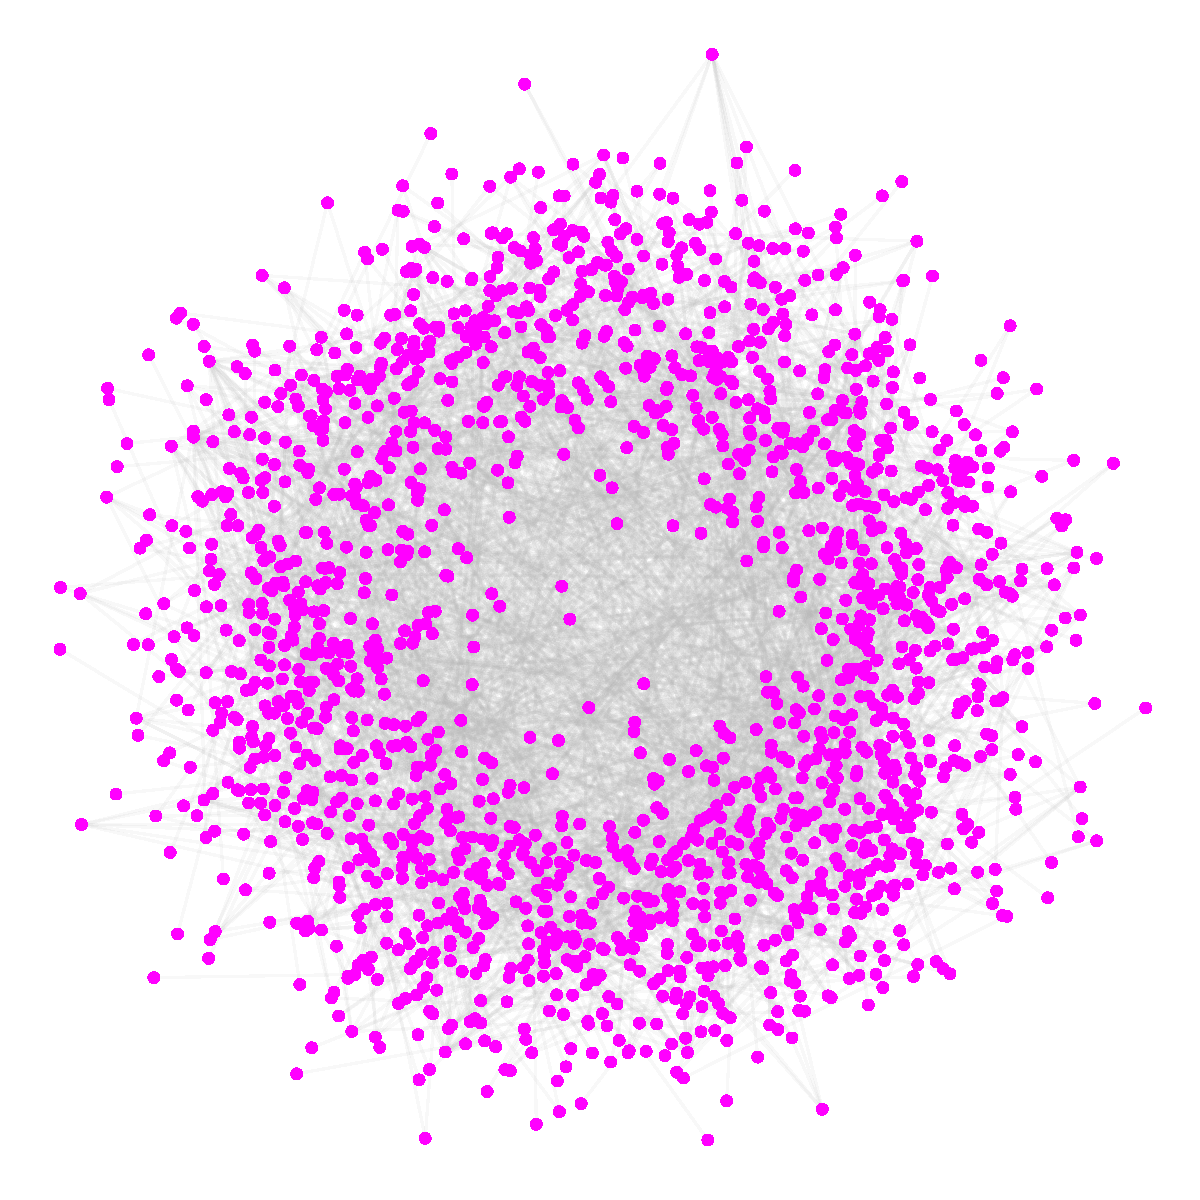
\includegraphics[width=.8\textwidth]{figure/yeast_geom_net-1.pdf}
\caption{\label{fig.cap:yeast} Protein-protein interaction network in \emph{S. cerevisiae}. A Fruchterman-Reingold algorithm allowed to run for 50,000 iterations produced the coordinates for the nodes.}
\end{figure}


\section{Some considerations of speed}\label{sec:speed}

In our examples thus far, we have focused on rather small social or relationship networks and one larger communication network. Now we present an example of a biological network, which comes from \citet{protein}. It is the complete protein-protein interaction network in the yeast species \emph{S. cerevisiae}. There are 2,113 proteins that make up the vertices of this network, with a total of 4480 edges between them.  These edges represent ``direct physical interactions" between any two proteins \citep[][p. 42]{protein}, resulting in a relatively large  network. When these interactions and their associated proteins are plotted using the Fruchterman-Reingold layout algorithm, the runtime is extremely long, about 9.5 minutes for 50,000 iterations through the algorithm. The resulting layout is shown in Figure~\ref{fig.cap:yeast}. When testing the three approaches with the larger network, we decided to use a random layout to save time. Despite its size, each one of the approaches in the \pkg{ggplot2} framework can be drawn in a few hundred milliseconds. 

Another benefit that emerges from using \pkg{ggplot2} for network visualization is the speed at which it can plot fairly large networks. In order to assess the speed gain procured by our three approaches, we ran two separate tests, both of which designate \pkg{ggplot2}-based approaches as faster than the plotting functionality offered in the \pkg{network} package. They also show the \pkg{ggplot2} approaches to be largely on par with the speed provided by the \pkg{igraph} package. We first investigate average random layout plotting time of the protein network 

shown in Figure~\ref{fig.cap:yeast}, and then consider average plotting times of increasingly larger random networks. Note that in all tests, default package settings were used. The code to create benchmark results for both of these situations is provided in the vignette of the package \CRANpkg{ggCompNet} \citep{ggCompNet}. See the Supplementary Material section at the end of this paper for more information. 

We plotted the protein interaction network of Figure~\ref{fig.cap:yeast} 100 times using the \pkg{network} and \pkg{igraph} packages, and compared their run times to 100 runs each of the three visualization approaches introduced in this paper. The results are shown in Figure~\ref{fig:timings}. We can see that on average, the \pkg{ggplot2} framework provides a two to three-fold increase in speed over the network package, and that \pkg{geomnet} and \pkg{ggnetwork} are faster than package \pkg{igraph}. The three \pkg{ggplot2} approaches also have considerably less variability in time than the \pkg{network} package.
Despite the large number of vertices, the protein interaction network has a relatively small number of edges (4480 out of over 2.2 million theoretically possible connections resulting in an edge probability of just over 0.0020). Next, we examine networks with a higher edge probability.

\begin{figure}[b]
\centering

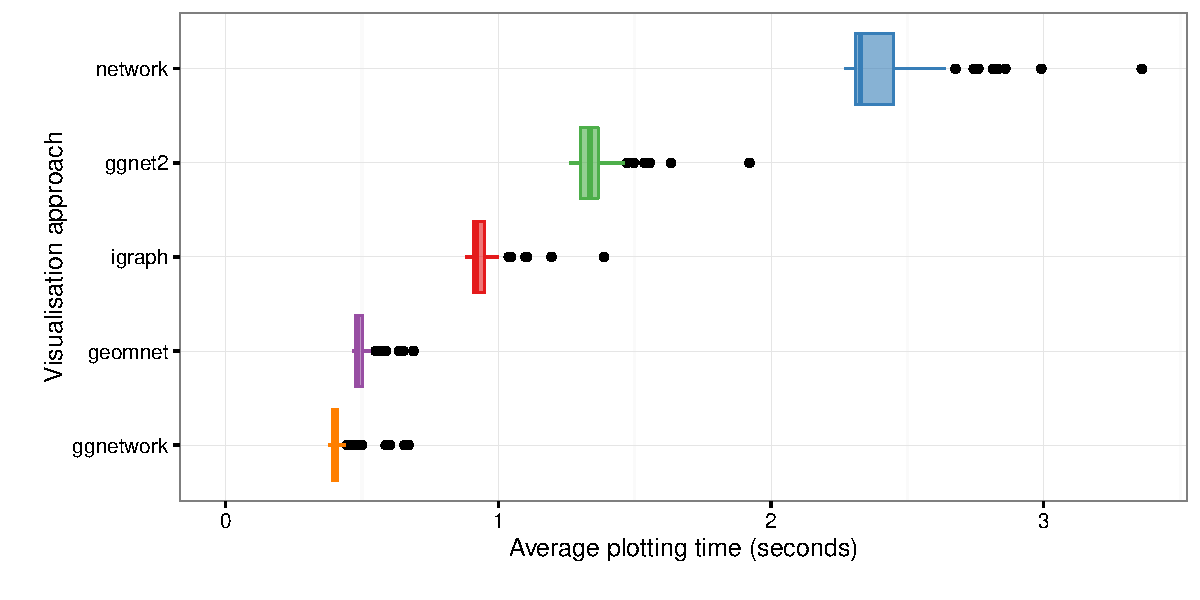
\includegraphics[width=\textwidth]{figure/compare-1.pdf}
\caption{\label{fig:timings} Comparison of the times needed for calculating and rendering the previously discussed protein interaction network in the three \pkg{ggplot2} approaches and the standard plotting routines  of the \pkg{network} and \pkg{igraph} packages based on 100 evaluations each.  }
\end{figure}

The second test relies on random undirected networks in which the probability of an edge between two nodes was set to $p = 0.2$. We generated 100 of these networks at network sizes from 25 to 250 nodes, using increments of 25.

\begin{figure}[hbtp]
\centering



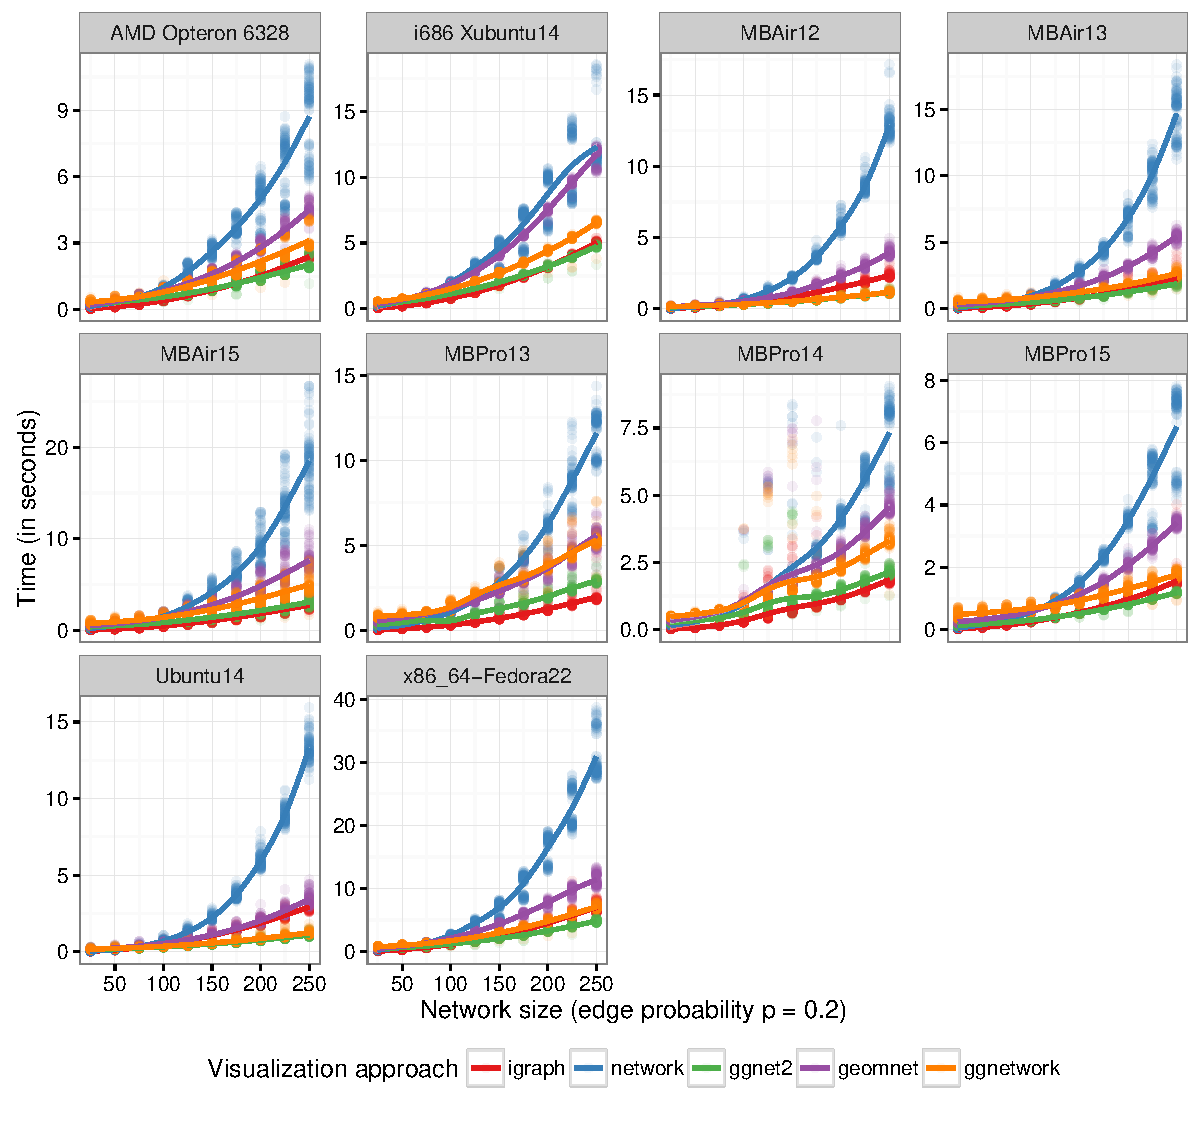
\includegraphics[width=\textwidth]{figure/runtimes-all-1.pdf}
\caption{\label{fig.cap:runtimes-random} Plotting times of random undirected networks of different sizes under each of the available visualization approaches using their default settings. Note that each panel is scaled independently to highlight relative differences in the visualization approaches rather than speed of different hardware.
}
\end{figure}

Figure~\ref{fig.cap:runtimes-random} summarizes the results of these benchmarks using a convenience sample of machines accessible to the authors, including authors' hardware and additional results from friends' and colleagues' machines.
Network sizes are plotted horizontally, execution times of 100 runs under each visualization approach are plotted on the $y$-axis. Each panel shows a different machine as indicated by the facet label. Note that each panel is scaled separately to account for differences in the overall speed of these machines.
What these plots indicate is that we have surprisingly large variability in relative run times across different machines.
However, the results support some  general findings.
The \pkg{network} plotting routine is by far the slowest across all machines, while the \pkg{igraph} plotting is generally among the fastest. Our three approaches generally feature in between \pkg{igraph} and \pkg{network} with \code{ggnet2} being as fast or faster than \pkg{igraph} plotting, followed by \pkg{ggnetwork} and \pkg{geomnet}, which is generally the slowest among the three. These differences become more pronounced as the size of the network increases.

Although speed was not the main rationale for our inquiry into \pkg{ggplot2}-based approaches to network visualization, a speed-based comparison shows a clear advantage of these approaches over the plotting function included in the \pkg{network} package, which very quickly becomes much slower as network size increases.

\section{Summary and discussion}

At first  glance, the three visualization approaches may seem nearly identical. However, each one brings unique strengths to the visualization of networks.  Out of our three approaches, \pkg{ggnetwork} is most flexible and allows for a re-ordering of layers to emphasize one over the other. The flexibility is useful but does require the user to specify every single part of the network visualization. The \pkg{geomnet} implementation most closely aligns with the existing \pkg{ggplot2} paradigm because it provides a single layer that can be added to other \code{ggplot2} layers. \code{ggnet2} requires the user to know the least about the \pkg{ggplot2} framework, while resulting in a valid and extensible \pkg{ggplot2} object. Many features of the packages would not have been possible, or would have at least been difficult to implement, in  prior versions of \pkg{ggplot2}.  The increased flexibility of the current development version as well as the added \code{geom}s \code{geom\_curve} and \code{geom\_label} provided us with a strong, yet flexible, foundation for network visualization. Our approaches also benefit from the speed of \pkg{ggplot2},  making network visualization more efficient than the existing framework of \pkg{network} for a lot of the benchmark examples.

All three approaches rely on the package \pkg{sna} for layouts. This allows the user to access the many layout algorithms available for networks, and in the event that new layouts are implemented in \pkg{sna}, our packages will accommodate them seamlessly. A larger range of layouts is available through \pkg{igraph}, and can be implemented into our packages by setting the respective layout arguments to \code{NULL} and passing \code{x,y} coordinates calculated from \pkg{igraph}. There are some notable differences between the packages, such as in the parameters used for specific layout algorithms, e.g.\ \pkg{igraph} allows the use of weights for Fruchterman-Reingold placement, even though it is unclear from the original article how these are supposed to affect the layout. In all  three approaches, it is  feasible to tap into \pkg{igraph}'s functionality in a future version so that the user does not need to calculate the layout separately. Additional future work will explore the implementation of other network data structures, such as the \code{networkDynamic} class from \pkg{statnet}, which would benefit from the faceting capabilities of our implementations. This work will likely incorporate the \code{fortify} approach of \pkg{ggnetwork} and \code{geomnet::fortify.network()} for converting network data structures to a \pkg{ggplot2}-friendly format.

We have found that none of our approaches is unequivocally the best. We can, however, provide some guidance as to which approach is best for which type of user. The main differences between the three methods are in the way that network information is passed into the functions. For \code{ggnet2} and \pkg{ggnetwork}, data management and attribute handling is done through network operators on nodes and edges, while the \pkg{geomnet} approach does not require any knowledge of networks or existing network analysis packages from the user. This likely affects the user base of each package. We think that users who are well-versed with networks will find \code{ggnet2} and \pkg{ggnetwork} more intuitive to use than \pkg{geomnet}. These users might be looking to \pkg{ggplot2} as another avenue to create high-quality visualizations that tap into \pkg{ggplot2} advantages such as facetting and, for \pkg{ggnetwork}, layering. Users who are already familiar with \pkg{ggplot2} and some of the other \CRANpkg{tidyverse} packages (see \citet{tidyverse}), and who find themselves dealing with network data will likely be more attracted to the \pkg{geomnet} implementation of network plotting. The data management skills needed for using \pkg{geomnet} are basic: some familiarity with the split-apply-combine paradigm, in the form of familiarity with \CRANpkg{plyr} or \CRANpkg{dplyr}, would be sufficient in order to make full use of the features of \code{geom\_net} \citep{plyr}. All in all, the three approaches we have presented here provide a wealth of resources to users of all skill sets who are looking to create beautiful network visualizations.

On a personal level we discovered that the collaboration on this paper has helped us to improve upon our initial versions of each of these packages. For instance, the edge coloring in the \code{ggnet2} function was designed so that edges between two vertices in the same group were colored with that group's vertex color. This  inspired an implementation of it in \code{geomnet} through the traditional \code{ggplot2} \code{group} operator. During the process of writing the paper the authors collaborated on a solution for the problem of nodes being plotted on top of arrow tips. This solution  was implemented in the \pkg{geomnet} \code{arrow.gap} parameter, which allows to re-track the tip of an arrow on a directed edge, and was also added to \pkg{ggnetwork}. In addition, the implementation of a \pkg{ggplot2} \code{geom} for networks within \pkg{geomnet} inspired the creation of the aliased \code{geom}s of the \pkg{ggnetwork} package. 

Finally, curious users may be interested in how these three packages can fit together and replicate each other, since they are in fact so similar. Thanks to the flexibility inherent to \pkg{ggnetwork}, it is possible to write wrapper functions around \pkg{ggnetwork} functions in order to recreate the behavior and functionality of \code{ggnet2} and \pkg{geomnet}. Simple examples of such wrapper functions, called \code{ggnetwork2} and \code{geom\_network}, respecively are shown below. 

\begin{knitrout}
\definecolor{shadecolor}{rgb}{1, 1, 1}\color{fgcolor}\begin{kframe}
\begin{verbatim}
library(ggnetwork)
# mimics geom_net behavior
geom_network <- function(edge.param, node.param) { 
     edge_ly <- do.call(geom_edges, edge.param) 
     node_ly <- do.call(geom_nodes, node.param) 
     list(edge_ly, node_ly) 
}
# mimics ggnet2 behavoir
ggnetwork2 <- function() { ggplot() + geom_network() }
\end{verbatim}
\end{kframe}
\end{knitrout}

Similarly, \pkg{geomnet} can mimic the the behavior of \code{ggnet2}, as shown below. 
\begin{knitrout}
\definecolor{shadecolor}{rgb}{1, 1, 1}\color{fgcolor}\begin{kframe}
\begin{verbatim}
library(geomnet)
geomnet2 <- function(net) { 
  ggplot(data = fortify(net),
         aes(from_id = from_id, to_id = to_id)) + 
    geom_net()
}
\end{verbatim}
\end{kframe}
\end{knitrout}

Mimicking \pkg{ggnetwork} with \pkg{geomnet} requires a little bit more work because the native data input for \pkg{geomnet} is a \code{"data.frame"} object fortified with \pkg{geomnet} methods, not a \code{"network"} object. Instead, the internal \pkg{ggplot2} function \code{ggplot\_build} allows a plot created with \pkg{geomnet} function calls to be recreated with \pkg{ggnetwork}-like syntax. An example of using a \pkg{geomnet} plot to create a similar plot in the style of \pkg{ggnetwork} follows to reproduce Figure~\ref{fig.cap:blood}(c).
\begin{knitrout}
\definecolor{shadecolor}{rgb}{1, 1, 1}\color{fgcolor}\begin{kframe}
\begin{verbatim}
library(geomnet)
library(ggnetwork)
library(dplyr)
# a ggnetwork-like creation using a geomnet plot 
data("blood")
# first, create the geomnet plot to access the data later
geomnetplot <- ggplot(data = blood$edges, aes(from_id = from, to_id =
                                                to)) +
                  geom_net(layout.alg = "circle", selfloops = TRUE) + 
                theme_net() 
# get the data
dat <- ggplot_build(geomnetplot)$data[[1]]
# ggnetwork-like construction for re-creating network shown in Figure 5 
ggplot(data = dat, aes(x = x, y = y, xend = xend, yend = yend)) + 
  geom_segment(arrow = arrow(type = 'closed'), colour = 'grey40') + 
  geom_point(size = 10, colour = 'darkred') +
  geom_text(aes(label = from), colour = 'grey80', size = 4) + 
  geom_circle() + 
  theme_blank() + theme(aspect.ratio = 1)
\end{verbatim}
\end{kframe}
\end{knitrout}

\begin{center}
{\large\bf Supplementary Material}
\end{center}

\begin{description}

\item[Software:] \pkg{ggnetwork} 0.5.1 and \pkg{geomnet} 0.2.0 were used to create the visualizations. \code{ggnet2} is part of \pkg{GGally} 1.3.0.

\item[Reproducibility:] All the code used in the examples is available as a vignette in the CRAN package \pkg{ggCompNet}. There are two vignettes: one for the speed comparisons and one for the visualizations provided in the Examples section. The package also provide our speed test data for creating Figure~\ref{fig.cap:runtimes-random}. We created this package to accompany this paper with the hope that interested users will compare these methods on their own systems and against their own code. Finally, all of the data we use in the examples, with the exception of the bipartite network example, is included as a part of the \pkg{geomnet} package. 

\end{description}

\begin{center}
{\large\bf Acknowledgements}
\end{center}

\begin{description}
\item The authors would like to thank the reviewers for their thoughtful input to and thorough reviews of our manuscript. We would also like to thank the editor of The R Journal for his enduring patience.  
\end{description}


\bibliography{tyner-briatte-hofmann}

\address{Samantha Tyner\\
  Department of Statistics and Statistical Laboratory\\
  Iowa State University\\
  United States\\}
\email{sctyner@mail.iastate.edu}

\address{Fran\c{c}ois Briatte\\
  European School of Political Sciences\\
  Catholic University of Lille\\
  France\\}
\email{francois.briatte@univ-catholille.fr}

\address{Heike Hofmann\\
  Department of Statistics and Statistical Laboratory\\
  Iowa State University\\
  United States\\}
\email{hofmann@mail.iastate.edu}

\end{article}

\end{document}
